\chapter{Forecasting the daily electricity consumption}
\label{cha:Forecasting the daily electricity consumption}
In this chapter the different forecasting techniques to perform a 24 hour prediction for an individual household are discussed. One daily prediction has a data granularity of an half hour, which means that $ 48 $ data points have to be estimated for each prediction. \\\textbf{update --> discussing data} The day we want to forecast is further indicated as the ``desired day''. 
First pre-processing is done in Section \ref{s:Pre-processing} and the time series used are discussed. Afterwards the baseline models are looked into in Section \ref{s:Baseline models}. These models are characterised by a low calculation load during training and they therefore serve as an easy to obtain result where a more complex model can be compared with. Next, more complex models based on a neural network philosophy are discussed in Section \ref{s:Neural network models}. ``Long Short-Term Memory'' and ``Gated Recurrent Unit'' are most suitable to process time series and therefore serve as the core model which is analysed with different design choices. Finally, a parameter search is conducted. Here, an analysis is made of the sensitivity of the choice of different parameters is made.\\
 
\section{Pre-processing}\label{s:Pre-processing}
The data that is available is summarized by Table \ref{tab:available_data}. 

\subsection{Data}
In order to reduce the calculation load to do the parameter search in Section \ref{s: Parameter search}, three series are selected from the \textit{consumption.csv} that is listed in Table \ref{tab:availablef_data}. The series are chosen based on the least missing values of the historic electrical consumption serie and the absence of a big shift. Figure \ref{fig:three_series} shows the three figures and Table \ref{tab:three_series} summarizes their characteristics.\\

\begin{figure}[ht]
	\begin{subfigure}{0.32\textwidth}
		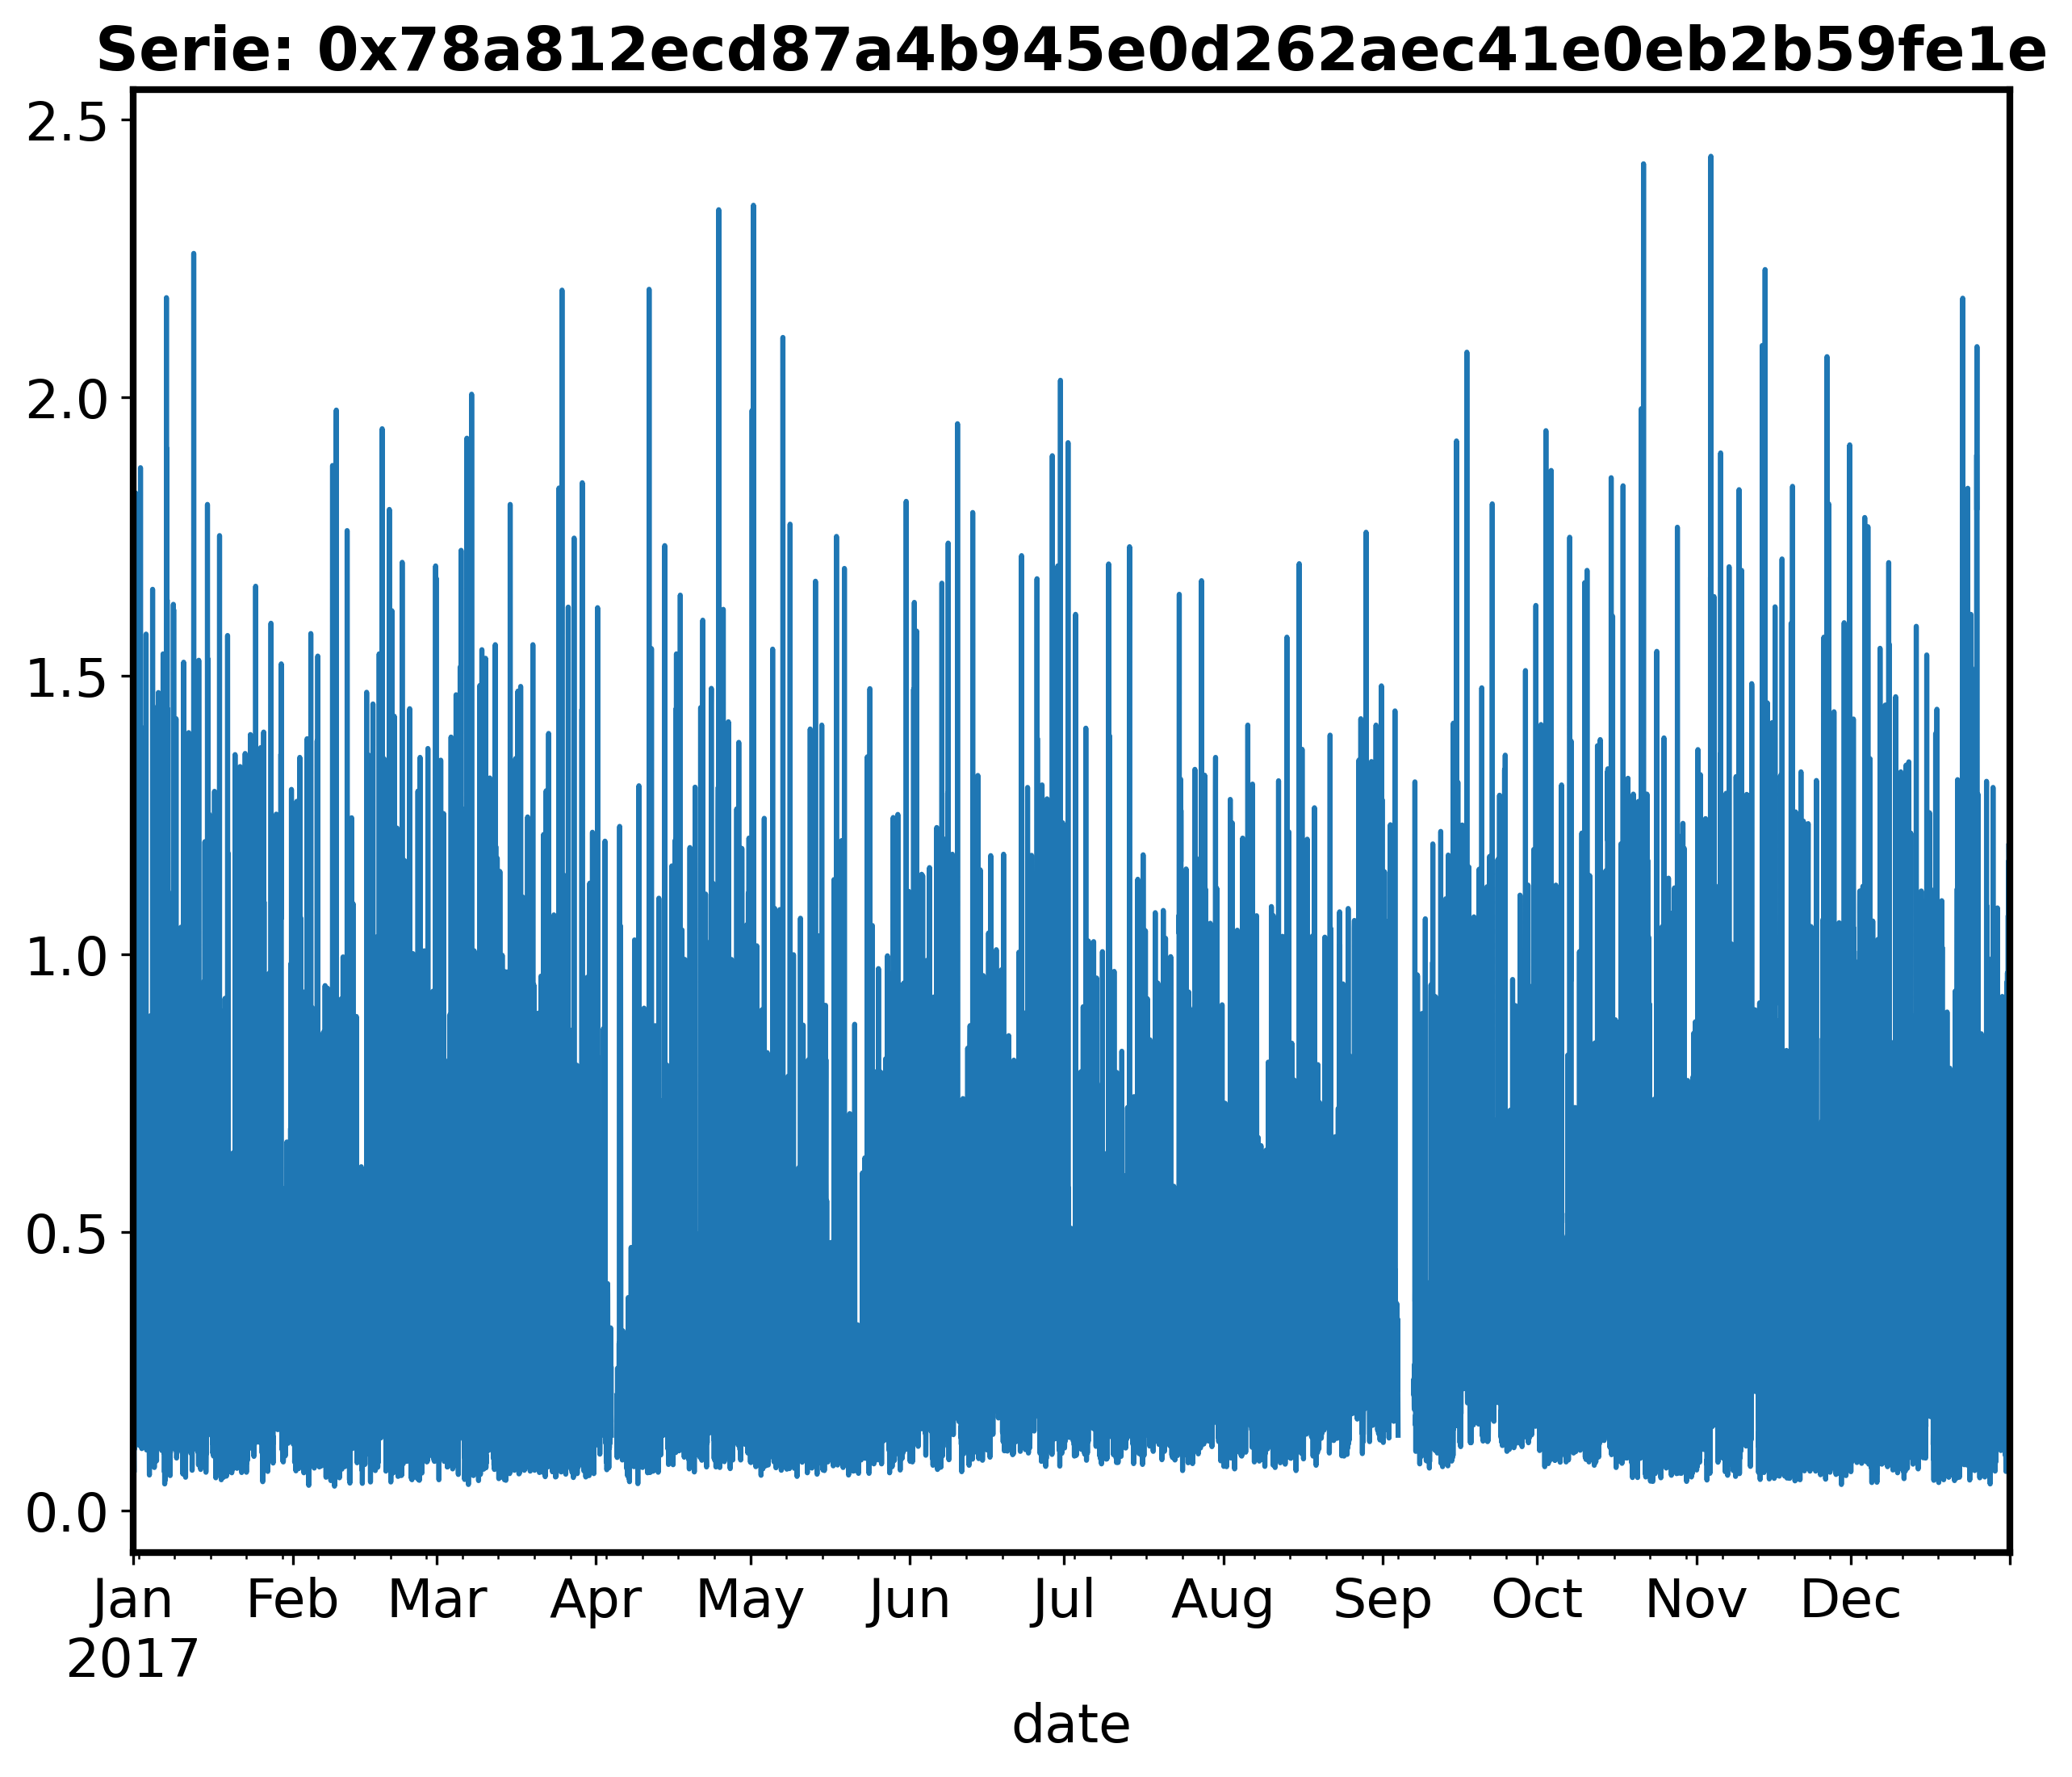
\includegraphics[width=1\linewidth]{Serie0x78a812ecd87a4b945e0d262aec41e0eb2b59fe1e.png}
		\caption{Serie $ 1 $}
	\end{subfigure}	 	
	\begin{subfigure}{0.32\textwidth}
		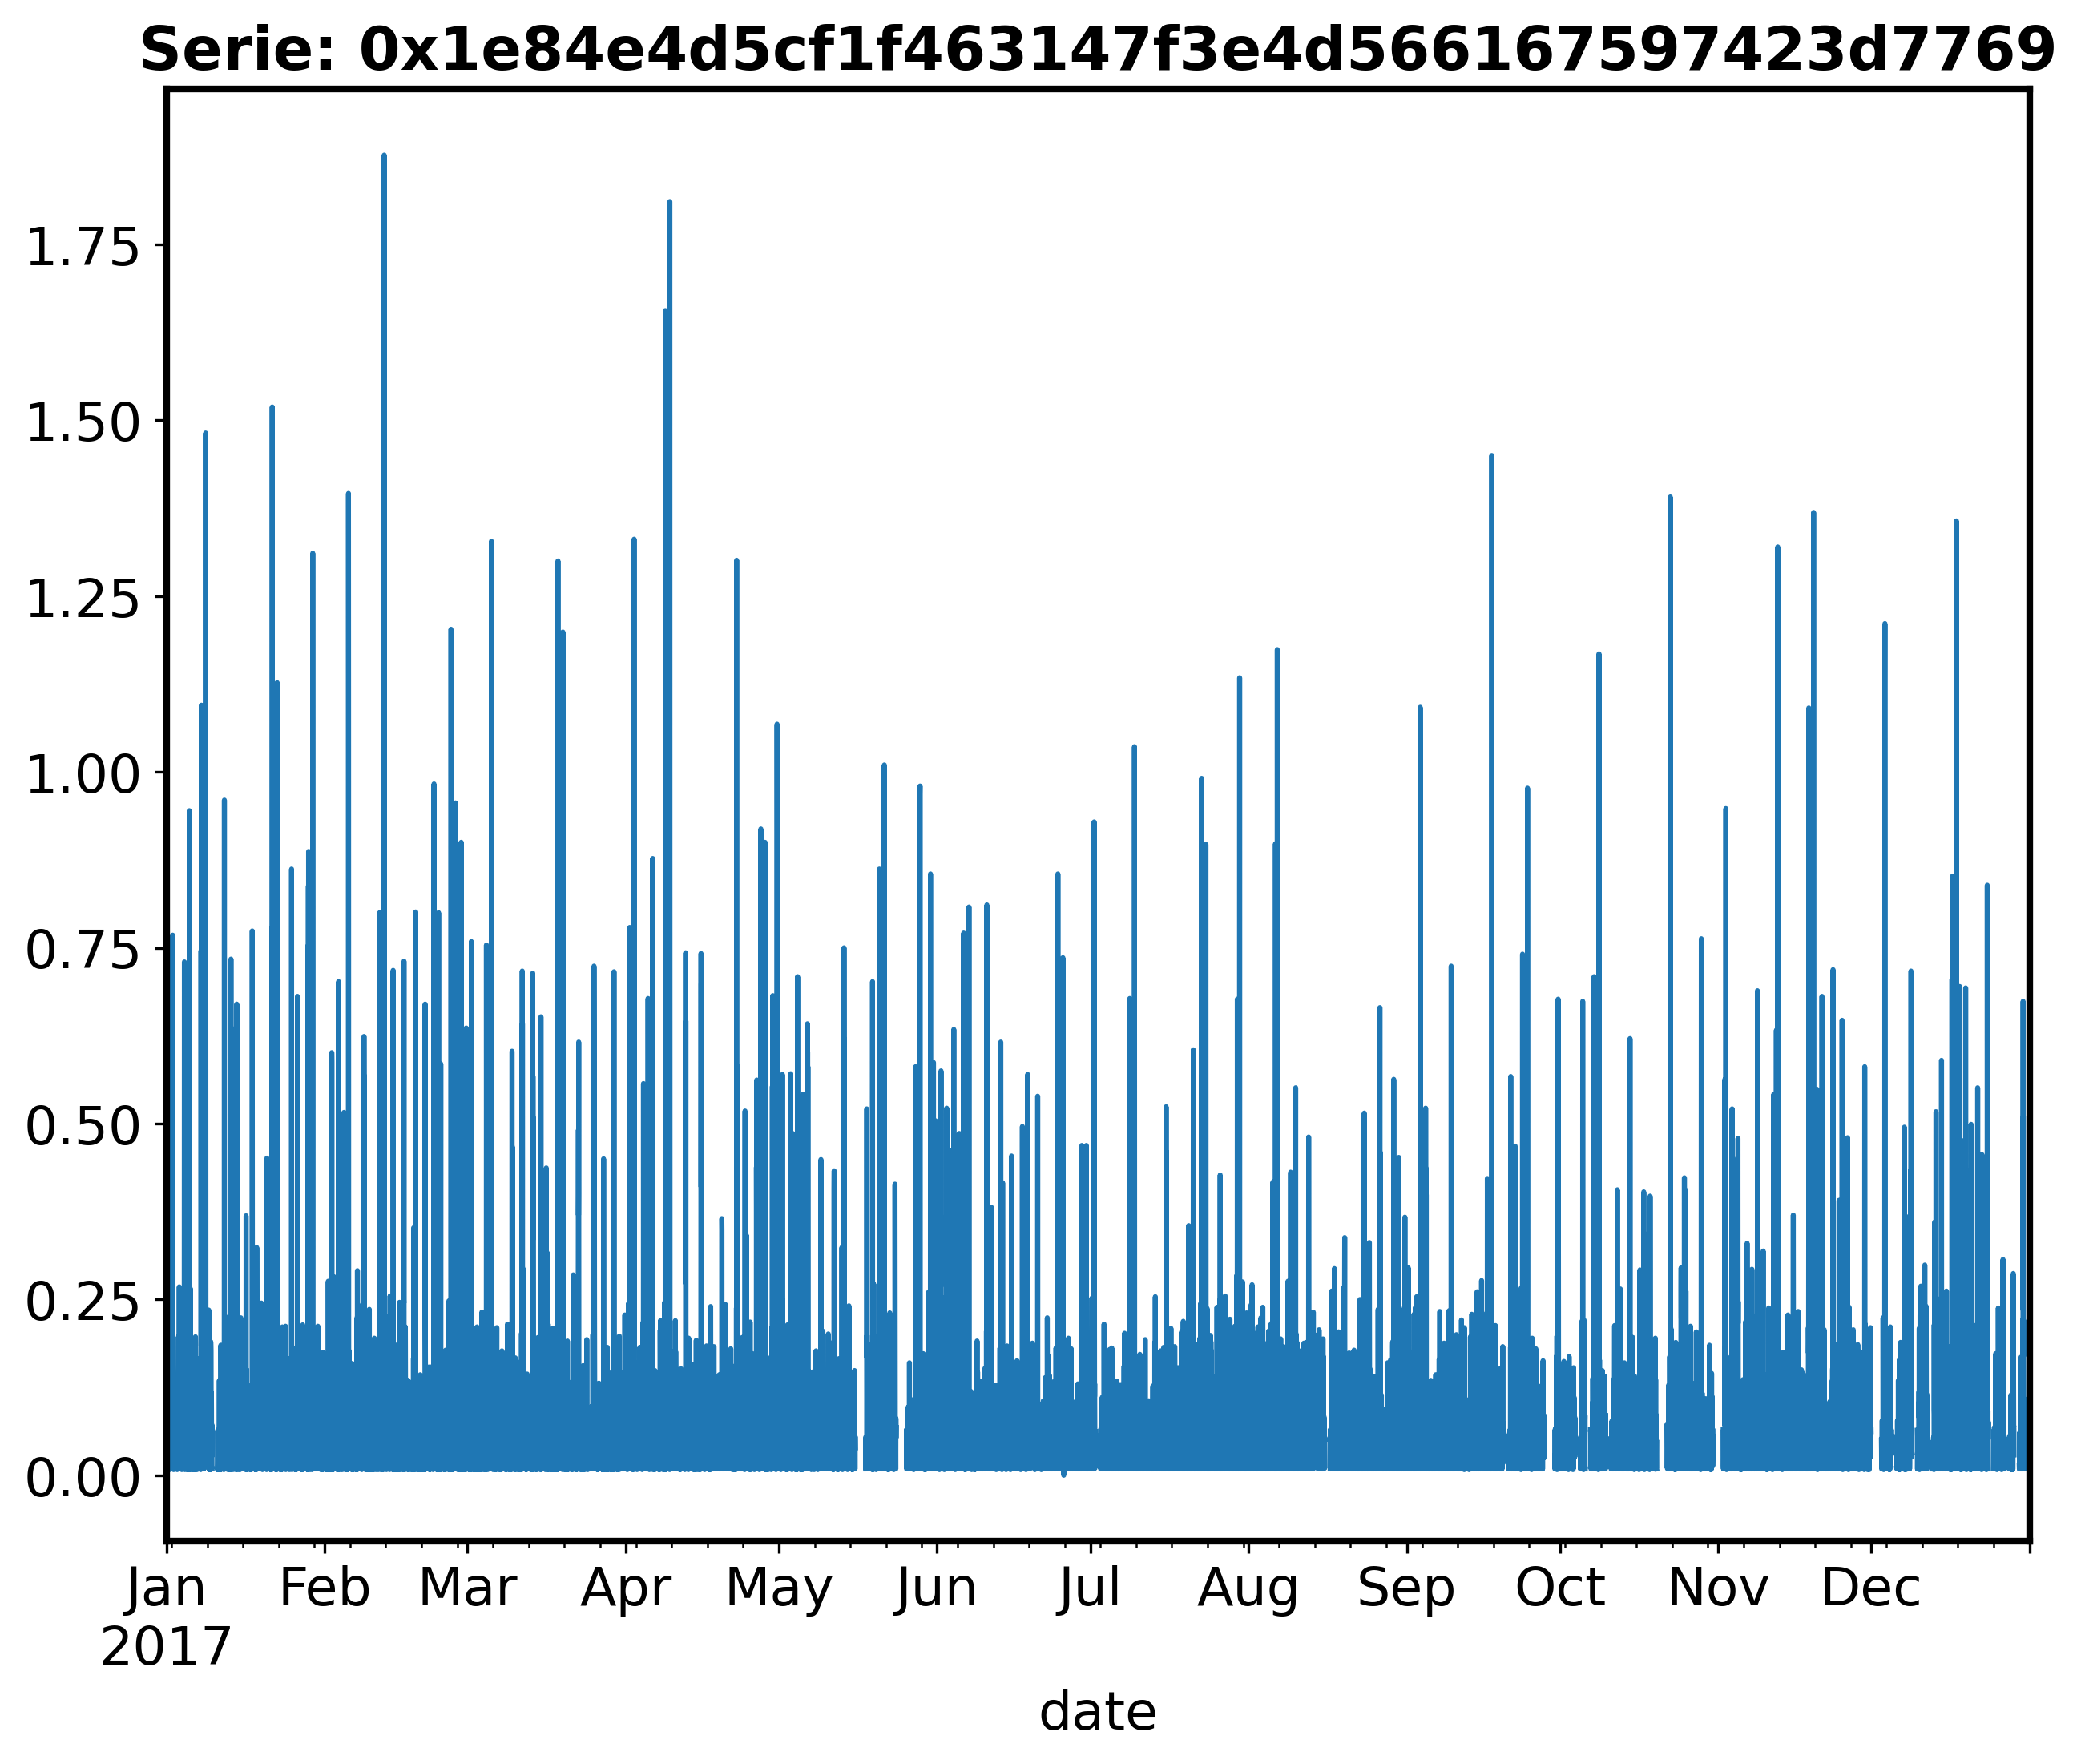
\includegraphics[width=1\linewidth]{Serie0x1e84e4d5cf1f463147f3e4d566167597423d7769.png}
		\caption{Serie $ 2 $}
	\end{subfigure}	
	\begin{subfigure}{0.32\textwidth}
		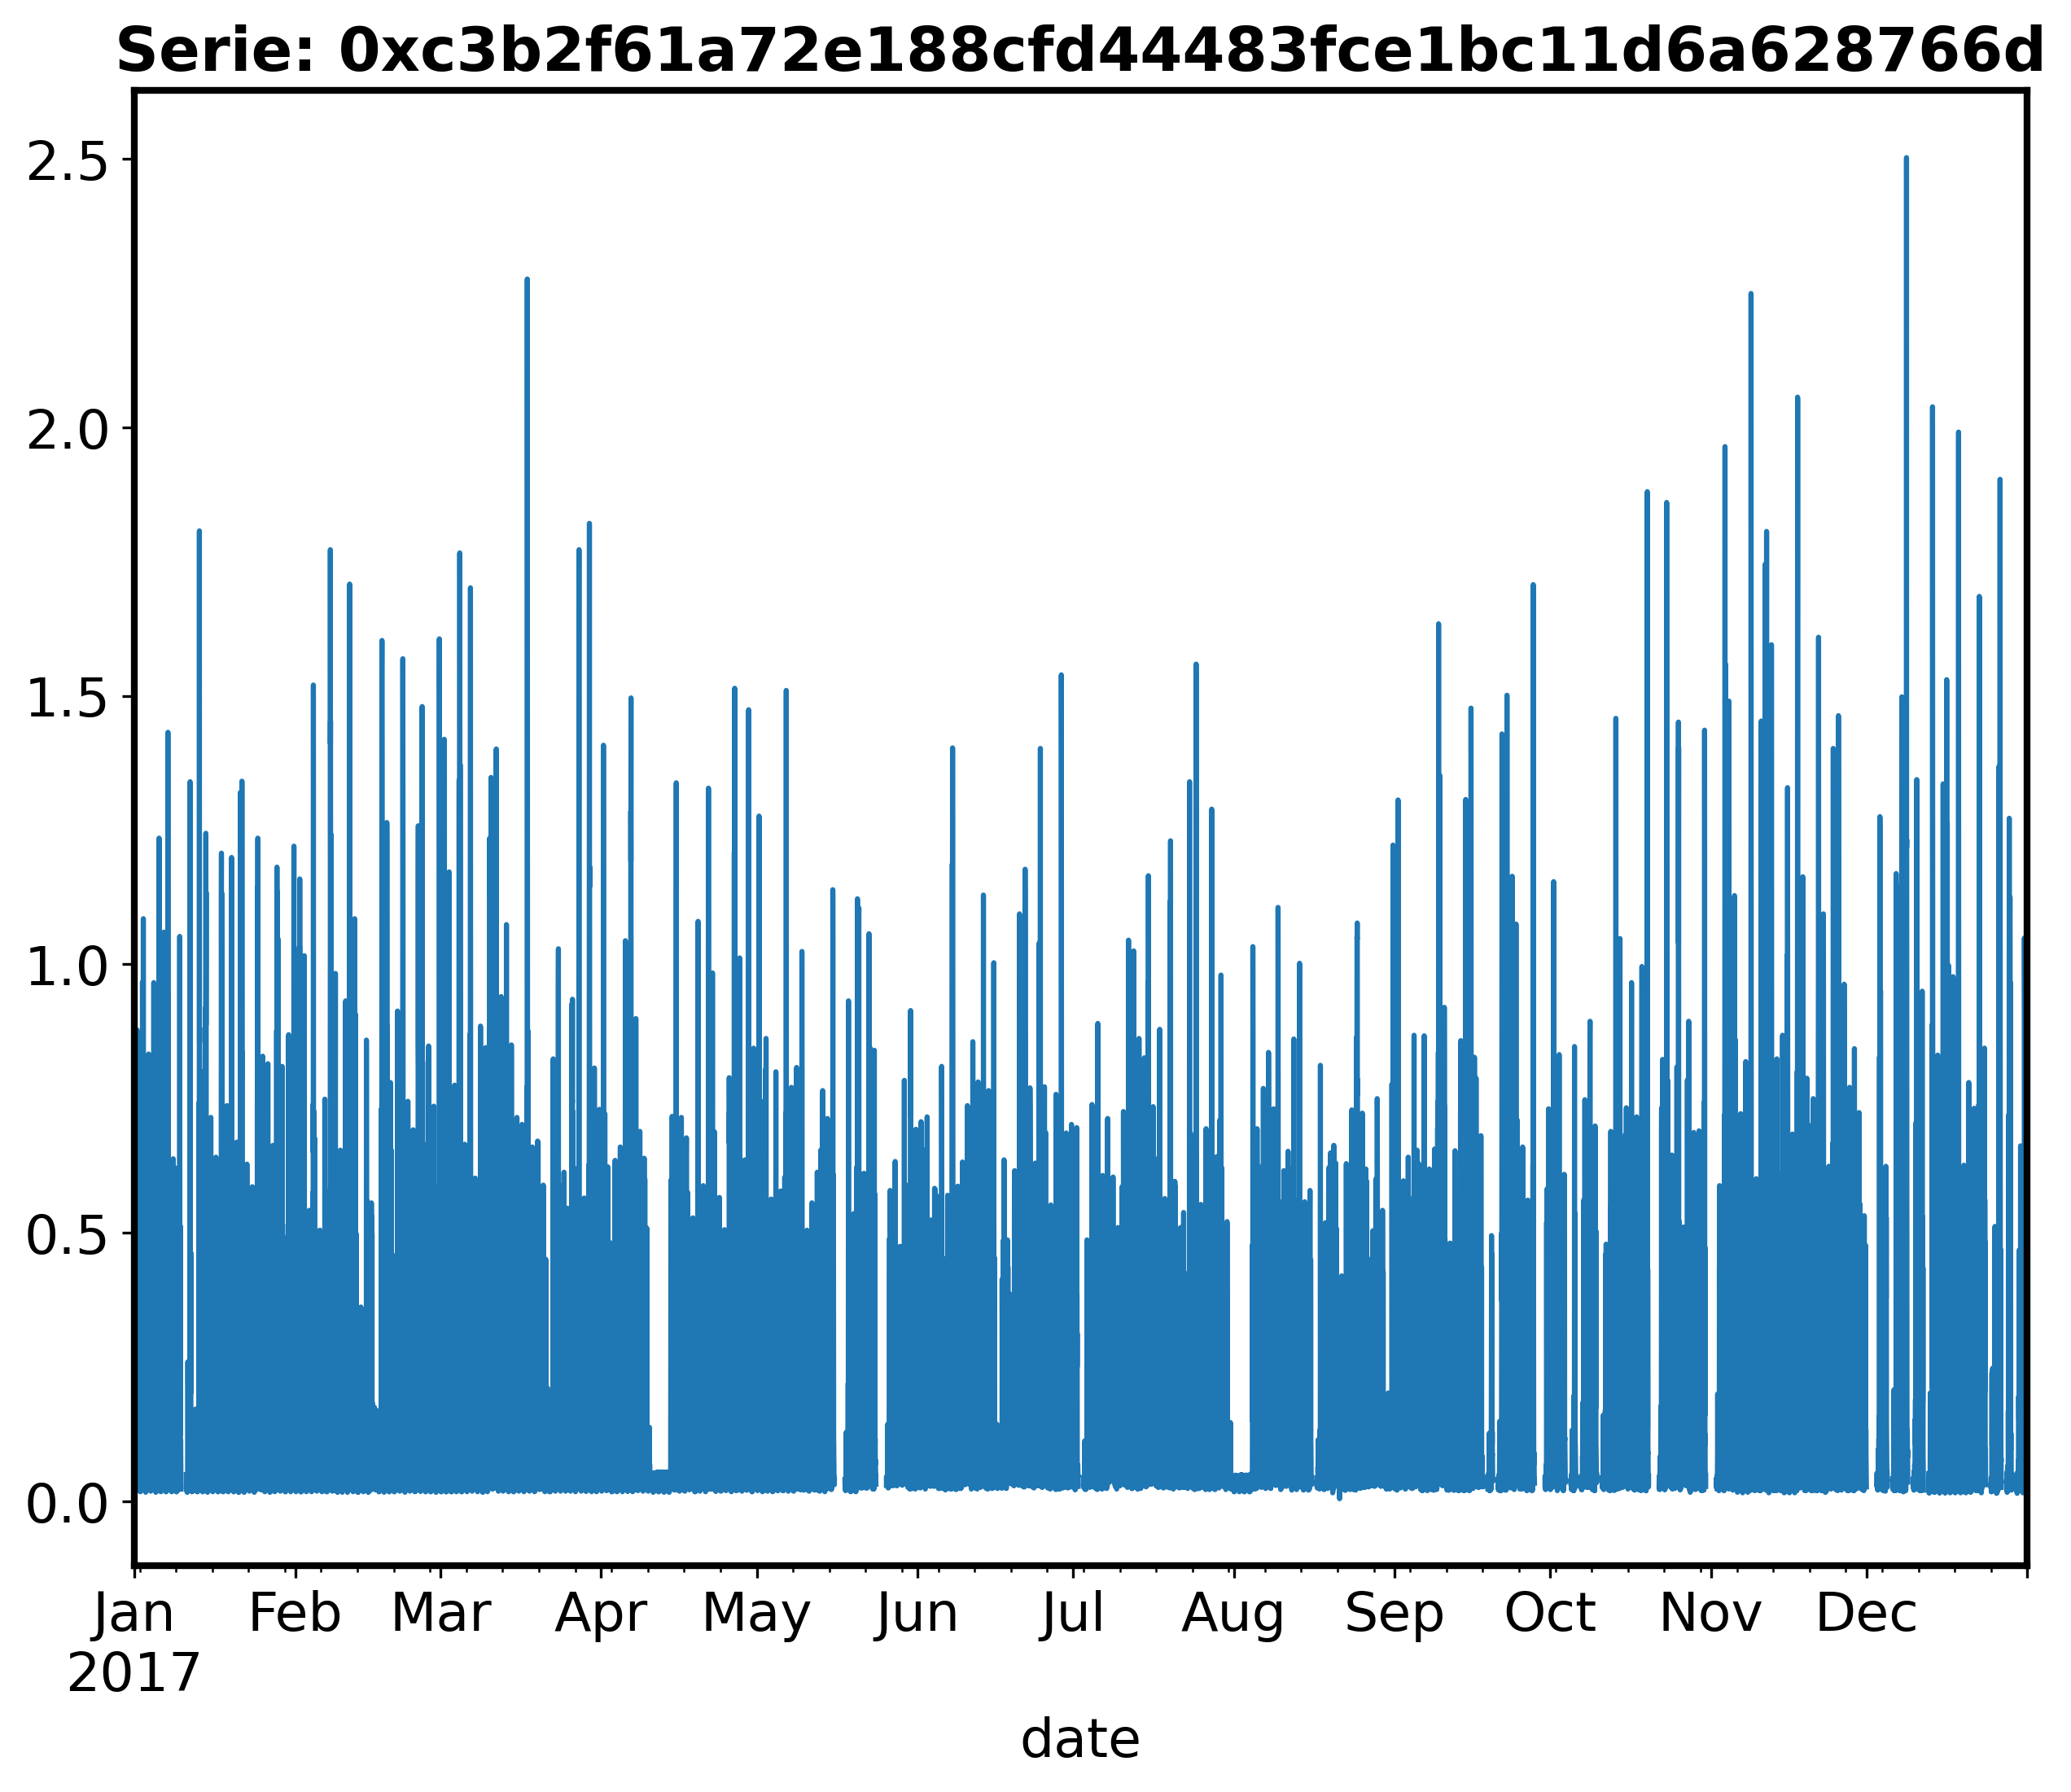
\includegraphics[width=1\linewidth]{Serie0xc3b2f61a72e188cfd44483fce1bc11d6a628766d.png}
		\caption{Serie $ 3 $}
	\end{subfigure}
	\caption{The consumption of $ 2017 $ for the three selected series. }
\end{figure}

\begin{table}
  \centering
  \begin{tabular}{@{}l|llr@{}} \toprule
  	\textbf{Characteristic}	& \textbf{Serie $ 1 $} & \textbf{Serie $ 2 $} & \textbf{Serie $ 3 $}\\\midrule
    Mean daily consumption [kWh]& $ 14.55 $&$ 3.17 $  & $ 6.58 $ \\
    Standard deviation daily consumption [kWh] &$ 3.21 $ & $ 0.99 $& $ 2.57 $ \\
    Median daily consumption [kWh] & $ 14.09 $ & $ 2.96 $& $ 5.88 $ \\
    Maximum daily consumption [kWh] & $ 30.08 $ & $ 6.60 $ &  $ 17.15 $   \\
    Minimum daily consumption [kWh]& $ 7.51 $ & $ 1.83 $ &  $ 1.50 $   \\
    Total missing days (consumption) & $ 4 $ &$ 25 $ & $ 26 $\\
    Days in validation set (November)&  $ 30 $ & $ 29 $  & $ 29 $ \\
    Days in Test set (December) & $ 31 $    &    $ 23 $  & $ 23 $ \\
    Days in training set (Rest)&   $ 300 $  &  $ 288 $   &  $ 287 $\\
    Mean average temperature [$\degree C$]& $ 10.37 $  &  $ 10.61 $  & $ 10.22 $ \\
    Standard deviation average temperature [$\degree C$]& $ 5.09 $  & $ 5.20 $   & $ 5.01 $ \\
    Median average temperature [$\degree C$] &  $ 10.46 $ &  $ 10.61 $  & $ 10.35 $ \\
    Maximum average temperature [$\degree C$] & $ 23.99 $  & $ 24.51 $   & $ 22.95 $ \\ 
    Minimum average temperature [$\degree C$] & $ -1.07 $  &  $ -1.28 $  & $ -1.42 $ \\
    Missing average temperature days &  $ 0 $ & $ 0 $  & $ 0 $  \\ 
    Amount of holidays in $ 2017 $ & $ 8 $  &  $ 8 $  & $ 8 $ \\\bottomrule
  \end{tabular}
  \caption{summarizing characteristics about the selected series.}
  \label{tab:summ_data}
\end{table}

The three time series are divided in a training, validation and test set. As validation and test set are respectively the months November and December chosen. Because in this chapter the time series are not aggregated to a single signal as was the case in Section \ref{s:Analysis} the min-max normalization can be used. The missing values in the consumption are substituted by making use of following baseline models in order: ``previous week'' model, ``previous day'' model and the mean model. When a baseline can't make a forecast because the data is not available, a next baseline model is used. Similar, the missing values of the temperature are substituted by first looking at the temperature yesterday, then tomorrow and as last the mean temperature.\\

The simulations that are done in the chapter are performed on a virtual machine through the Microsoft Azure service.
Table \ref{tab:CPU} shows the different features of the hired machine. 
\begin{table}[hb]
	\centering
	\begin{tabular}{|p{5cm}||p{2cm}|p{2cm}|p{2cm}|p{2cm}|}\hline
		\textbf{Name}	& \textbf{Logical cores} & \textbf{RAM (GB)} & \textbf{Storage (GB)} & \textbf{Cost}\\\hline
		F4s v2 (CPU - Azure)& $ 4 $&$ 8 $  & $ 32 $ & $ \$ 0.194/hour $\\\hline
		NVIDIA Tesla K80 (GPU - Azure)& $ 6 $&$ 56 $  & $ 380 $ & $\$ 1.166/hour$\\\hline
		i7-5500U@ $ 2.40 $ GHz (CPU - local) & $ 4 $ & $ 12 $ & $ 32 $ & $ - $\\\hline
	\end{tabular}
	\caption{Specifications of different CPU's and GPU tried.}
	\label{tab:CPU}
\end{table}


\textbf{- Make a table that summarizes the environment to do simulations.(baseline and othe models) (can be put in the appendix)}
\section{Baseline models}\label{s:Baseline models}
\subsection{Models}
As earlier discussed, the baseline models are characterised by a low calculation load during training and therefore serve as a baseline to compare more complex models with. The different baseline models tried are listed as follows:
\begin{itemize}
	\item Model 1: ``closest day forecast''
	\item Model 2: ``1 day ago forecast''
	\item Model 3: ``7 days ago forecast''
	\item Model 4: ``Mean forecast''
	\item Model 5: ``MAPE forecast''
\end{itemize} 

For all the models listed here, the training set for the forecast of the next day are all the days before this day of the year $ 2017 $. These models can therefore be categorized as ``lazy learning models'' because they only do work when they are asked a query. In contrast, the models discussed in Section \ref{s:Neural network models} generalize the training data without knowing the actual query. They belong to the ``eager learning methods'' class. The 24 hour predictions made by the $ 5 $ models are done all at once. This is in contrast to the models described in Section \ref{s:Neural network models}, where the prediction is made sample per sample and where the predictions done for an earlier hour of the day are taken into account.\\

\textbf{Model 1: ``closest day forecast''}\\
This model looks for the most similar day in the training set based on following metrics to make a prediction:

\begin{itemize}
	\item Holiday
	\item Day of the week
\end{itemize}

 All the days in the training are categorized according to these metrics. Then it is looked in which category the desired day belongs i.e. which day of the week and if it is a holiday. Inside the selected category, an assessment of the difference in average temperature is made for all days with respect to the desired day. It is assumed that the average temperature of the desired day is already available, which is a very plausible assumption. Finally, the day with the closest euclidean distance in temperature is selected and the electrical consumption signal is copied to serve as the prediction of the desired day. It should be noted that there are only a maximum of $ 8 $ holidays as can be seen in Table \ref{tab:summ_data}. Therefore, when a holiday should be predicted all Sundays are also included in the training set because a Sunday behaves most similar to a holiday as can be seen in Figure \ref{fig:sim_weekdays}.\\
 
 \textbf{Model 2: ``1 day ago forecast''}\\
 This model simply looks at the consumption of the day before the desired day. The philosophy of the model is that the most recent consumption data serves as a a good predictor.
 
 \textbf{Model 3: ``7 days ago forecast''}\\
 This model looks at the most recent household consumption of the previous corresponding day of the week. It is expected that people have a reasonably fixed routine during the week and therefore it is likely that this routine will also be found back in the electrical consumption.\\
 
 \textbf{Model 4: ``Mean forecast''}\\
 In the mean forecast the different days are again categorized as was done in Model $ 1 $, but instead of selecting a single day out of the group of days, a mean day is calculated and used as prediction of the desired day. No extra Sundays are included to forecast a holiday.\\
 
 \textbf{Model 5: ``MAPE forecast'' }\\
 This model solves for each half hour of the desired day a small non-linear optimization problem displayed by (Eq. \ref{eq:model_mape}). This model served as baseline model in paper \cite{Kong2019}. 
 
 \begin{equation}\label{eq:model_mape}
 	objective = \sum_{i=1}^K \zeta_{pi}\abs{\frac{(\hat{y}-p_i)}{pi}}
 \end{equation}
 
 Again a group of days of size $ M $, corresponding the desired day is selected based on the metrics of weekday and if the desired day is a holiday. Also Sundays are added to the group of holidays for this model. Next, the consumption at time $ t $ is extracted out of this group of days, which gives a list of length $ M $ with historic consumption values. From these values an empirical probability mass function $ \zeta_{pi} $ is derived by making use of a histogram using ``Freedman-Diaconis rule'' to decide the bin size. Figure \ref{fig:histogram_mape} shows an example of such an histogram. The amount of discretized values $ p_i $ is equal to the $ K $ bins and taken as the midpoint of two bin edges. From the count in the histogram the probability mass function for each discretized value is found. $ \hat{y} $ is found by minimizing equation \ref{eq:model_mape}.\\
 
The metrics used to evaluate the predictions performance of the baseline models are $ RMSE $ (Eq. \ref{eq:RMSE}), $ NRMSE $ (Eq. \ref{eq:NRMSE}), $ MAE $ (Eq. \ref{eq:MAE}), $ MSE $ (Eq. \ref{eq:MSE}) and $ MAPE $ (Eq. \ref{eq:MAPE}).

\begin{equation}\label{eq:MSE}
	MSE = \frac{\sum_{t=1}^{N}(\hat{y}_t-y_t)^2}{N}
\end{equation}

\begin{equation}\label{eq:MAPE}
	MAPE = \frac{\sum_{t=1}^{N}\abs{\hat{y}_t-y_t}/y_t}{N}
\end{equation}


It is expected that the \textit{MAE} punishes prediction errors more proportional than the \textit{MSE}, which takes the error squared. When an outlier occurs, $ MSE $ will see this as a bigger error than $ MAE $ does. The downside of using the absolute function is that it is not a smooth function. The advantage of using $ RMSE $ and $ MAE $ is that both have an error in kWh which is intuitive. $ NRMSE $ and $ MAPE $ take also the signal to predict into account. $ NRMSE $ gives a bigger error, when the true signal has not a lot of variation. $ MAPE $ takes into account that a small error value of on a signal with small amplitude has more impact than a small error on a signal with a big amplitude. Therefore, the latter is considered as a smaller error.


\subsection{Results of baseline models}
The results of the different forecasts of the month December are summarized by Table \ref{tab:summ_data_serie1}, \ref{tab:summ_data_serie2} and \ref{tab:summ_data_serie3}. In order to make a fair comparison only the days of December where all models could produce a forecast are included in the error metrics. 

\begin{table}[ht]
	\centering
	\begin{tabular}{@{}l|ccccr@{}} \toprule
		\textbf{Error metric}	& \textbf{Closest day} & \textbf{$ 1 $ day} & \textbf{$ 7 $ days} & \textbf{mean} & \textbf{MAPE}\\\midrule
		Mean absolute error& \cellcolor{red!25}$0.2049 $&$ 0.1954 $  & $0.1896 $ & \cellcolor{green!25}$ 0.1542 $ & $ 0.1920 $\\
		Mean squared error& \cellcolor{red!25}$0.1148 $&$ 0.1090 $  & $0.1011 $ & \cellcolor{green!25}$ 0.0701 $ & $ 0.1079 $\\
		Normalized root mean squared error& \cellcolor{red!25}$0.1591 $&$ 0.1550$  & $0.1493$ & \cellcolor{green!25}$ 0.1243$ & $ 0.1542$\\
		Root mean square error&\cellcolor{red!25} $0.3389 $&$ 0.3302$  & $0.3180$ & \cellcolor{green!25}$ 0.2648$ & $ 0.3285$\\
		Mean absolute percentage error & $ 0.5709 $&\cellcolor{red!25}$ 0.6163 $  & $ 0.5840 $ & $ 0.4594 $ & \cellcolor{green!25}$ 0.4138 $\\\bottomrule
	\end{tabular}
	\caption{Evaluation results for Serie $ 1 $ tested on $ 31 $ days of December.}
	\label{tab:summ_data_serie1}
\end{table}
% @{} just makes sure that the cell does not go further than the end of the text.
% c = center of cell, l = left, r = right
\begin{table}[ht]
	\centering
	\begin{tabular}{@{}l|ccccr@{}} \toprule
		\textbf{Error metric}	& \textbf{Closest day} & \textbf{$ 1 $ day} & \textbf{$ 7 $ days} & \textbf{mean} & \textbf{MAPE}\\\midrule
		Mean absolute error& $0.0559 $&\cellcolor{red!25}$ 0.0750 $  & $0.0693 $ & \cellcolor{green!25}$ 0.0473 $ & $ 0.0507 $\\
		Mean squared error& $0.0123 $&\cellcolor{red!25}$ 0.0264 $  & $0.0188 $ & \cellcolor{green!25}$ 0.0085 $ & $ 0.0125 $\\
		Normalized root mean squared error& $0.0823 $&\cellcolor{red!25}$ 0.1205$  & $0.1017$ & \cellcolor{green!25}$ 0.0681$ & $ 0.0828$\\
		Root mean square error& $0.1111 $&$ 0.1625$  &\cellcolor{red!25} $0.1373$ & \cellcolor{green!25}$ 0.0919$ & $ 0.1117$\\
		Mean absolute percentage error & $ 1.601 $&$ 2.1993 $  &\cellcolor{red!25} $ 2.3123 $ & $ 1.6657 $ & \cellcolor{green!25}$ 0.7841 $\\\bottomrule
	\end{tabular}
	\caption{Evaluation results for Serie $ 2 $ tested on $ 12 $ days of December.}
	\label{tab:summ_data_serie2}
\end{table}

\begin{table}[ht]
	\centering
	\begin{tabular}{@{}l|ccccr@{}} \toprule
		\textbf{Error metric}	& \textbf{Closest day} & \textbf{$ 1 $ day} & \textbf{$ 7 $ days} & \textbf{mean} & \textbf{MAPE}\\\midrule
		Mean absolute error& $0.1267 $&\cellcolor{red!25}$ 0.1370 $  & $0.1323 $ &\cellcolor{green!25} $ 0.1038 $ & $ 0.1130 $\\
		Mean squared error& $0.0824 $&$ 0.0846 $  & \cellcolor{red!25}$0.0895 $ & \cellcolor{green!25}$ 0.0521 $ & $ 0.0743 $\\
		Normalized root mean squared error& $0.1453 $&$ 0.1472$  & \cellcolor{red!25}$0.1514$ & \cellcolor{green!25}$ 0.1155$ & $ 0.1380$\\
		Root mean square error& $0.2871 $&$ 0.2909$  & \cellcolor{red!25}$0.2991$ & \cellcolor{green!25}$ 0.2282$ & $ 0.2726$\\
		Mean absolute percentage error & $ 0.8609 $&\cellcolor{red!25}$ 1.3153 $  & $ 0.9271 $ & $ 0.8094  $ &\cellcolor{green!25} $ 0.4792 $\\\bottomrule
	\end{tabular}
	\caption{Evaluation results for Serie $ 3 $ tested on $ 12 $ days of December.}
	\label{tab:summ_data_serie3}
\end{table}

% if mape performs best for the mape metric --> use both mean and mape as baseline models
The rule that the mean forecast outperforms the other methods can be concluded out of all the above tables when not looking to the MAPE metric. The order of the other forecasting techniques are in this case more serie dependent. The MAPE minimization technique logically performs for all time series best on the MAPE error metric. The mean forecast and the MAPE forecast will consequently be the models that are chosen as baseline models. It can be seen by inspecting the predictions that model $ 1 $,$ 2 $ and $ 3 $, which copy the consumption of another day, show more peaks in their prediction than model $ 4 $ and $ 5 $ that make use of the mean and MAPE techniques. Predictions of of the last mentioned models can be seen in Figure \ref{fig:baseline models 4 and 5} Also, a practical downside of model $ 1 $,$ 2 $ and $ 3 $ is that it is possible that they give no output e.g. when no temperature or consumption yesterday is available. \\

\begin{figure}[ht]
	\begin{subfigure}{0.5\textwidth}
		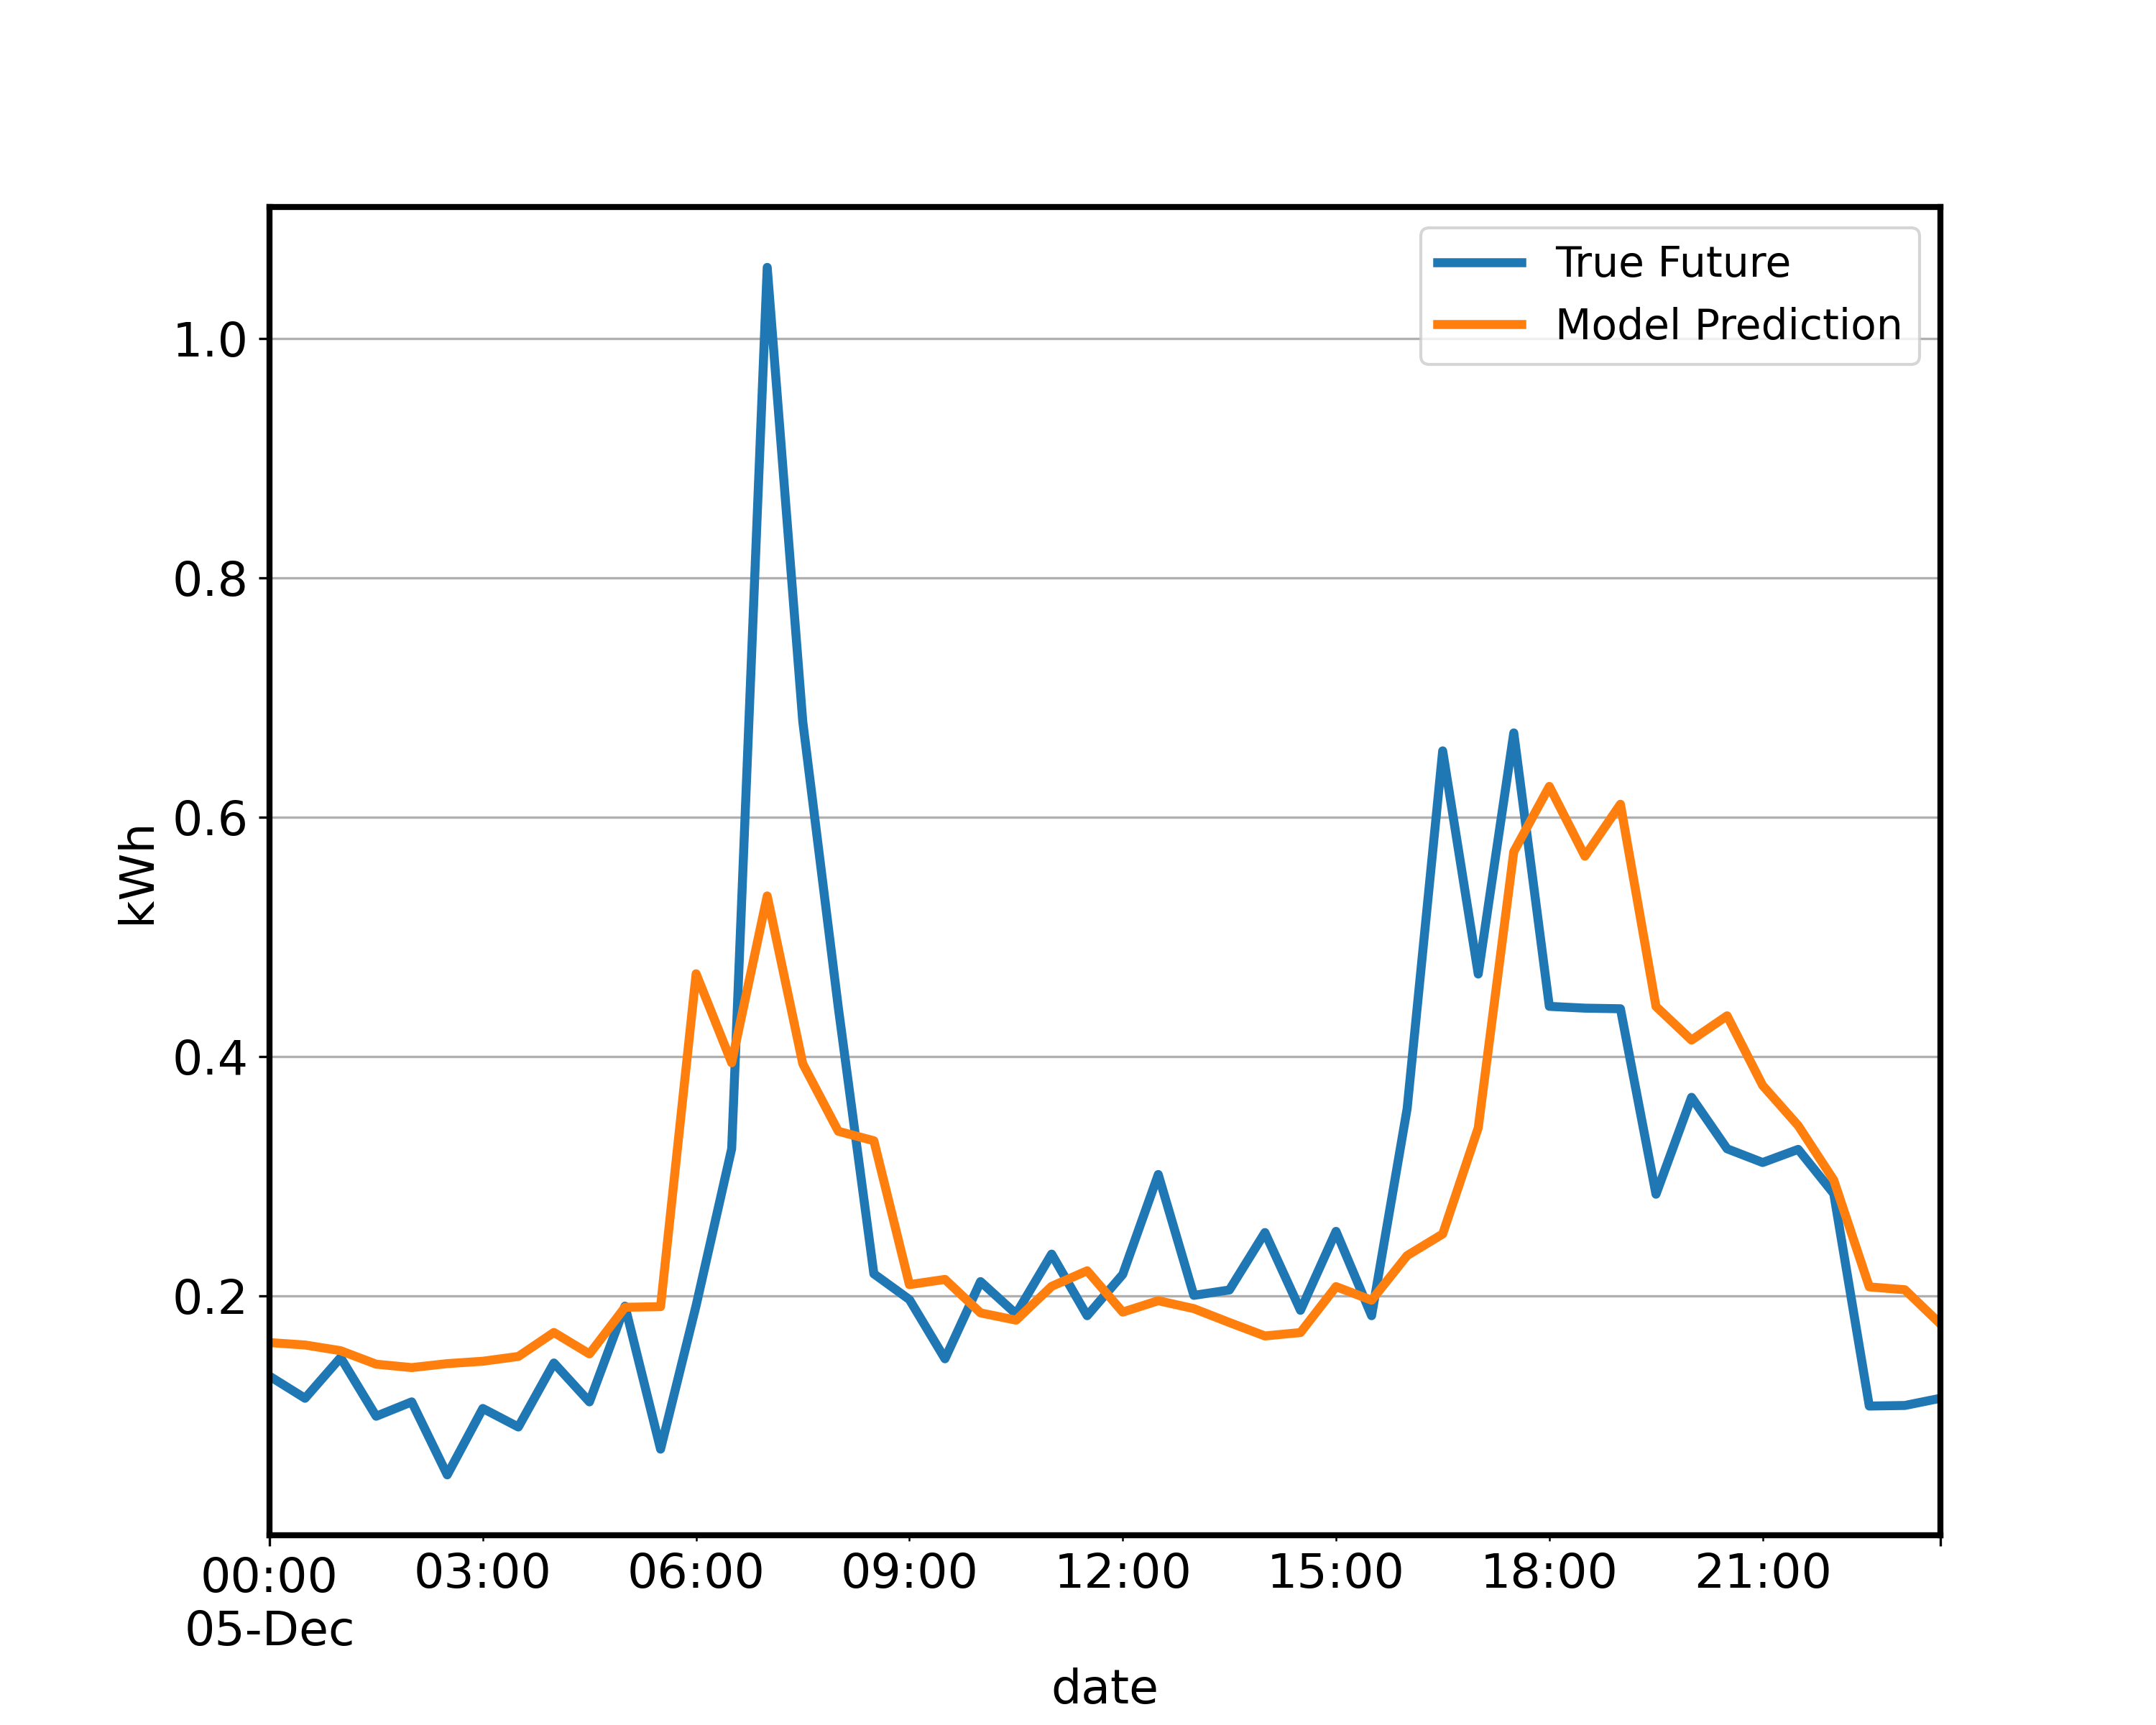
\includegraphics[width=1\linewidth]{mean_ID0x78a812ecd87a4b945e0d262aec41e0eb2b59fe1e_Day339_pred.png_1618425095.png}
		\caption{Model 4: ``Mean forecast''}
	\end{subfigure}	
	\begin{subfigure}{0.5\textwidth}
		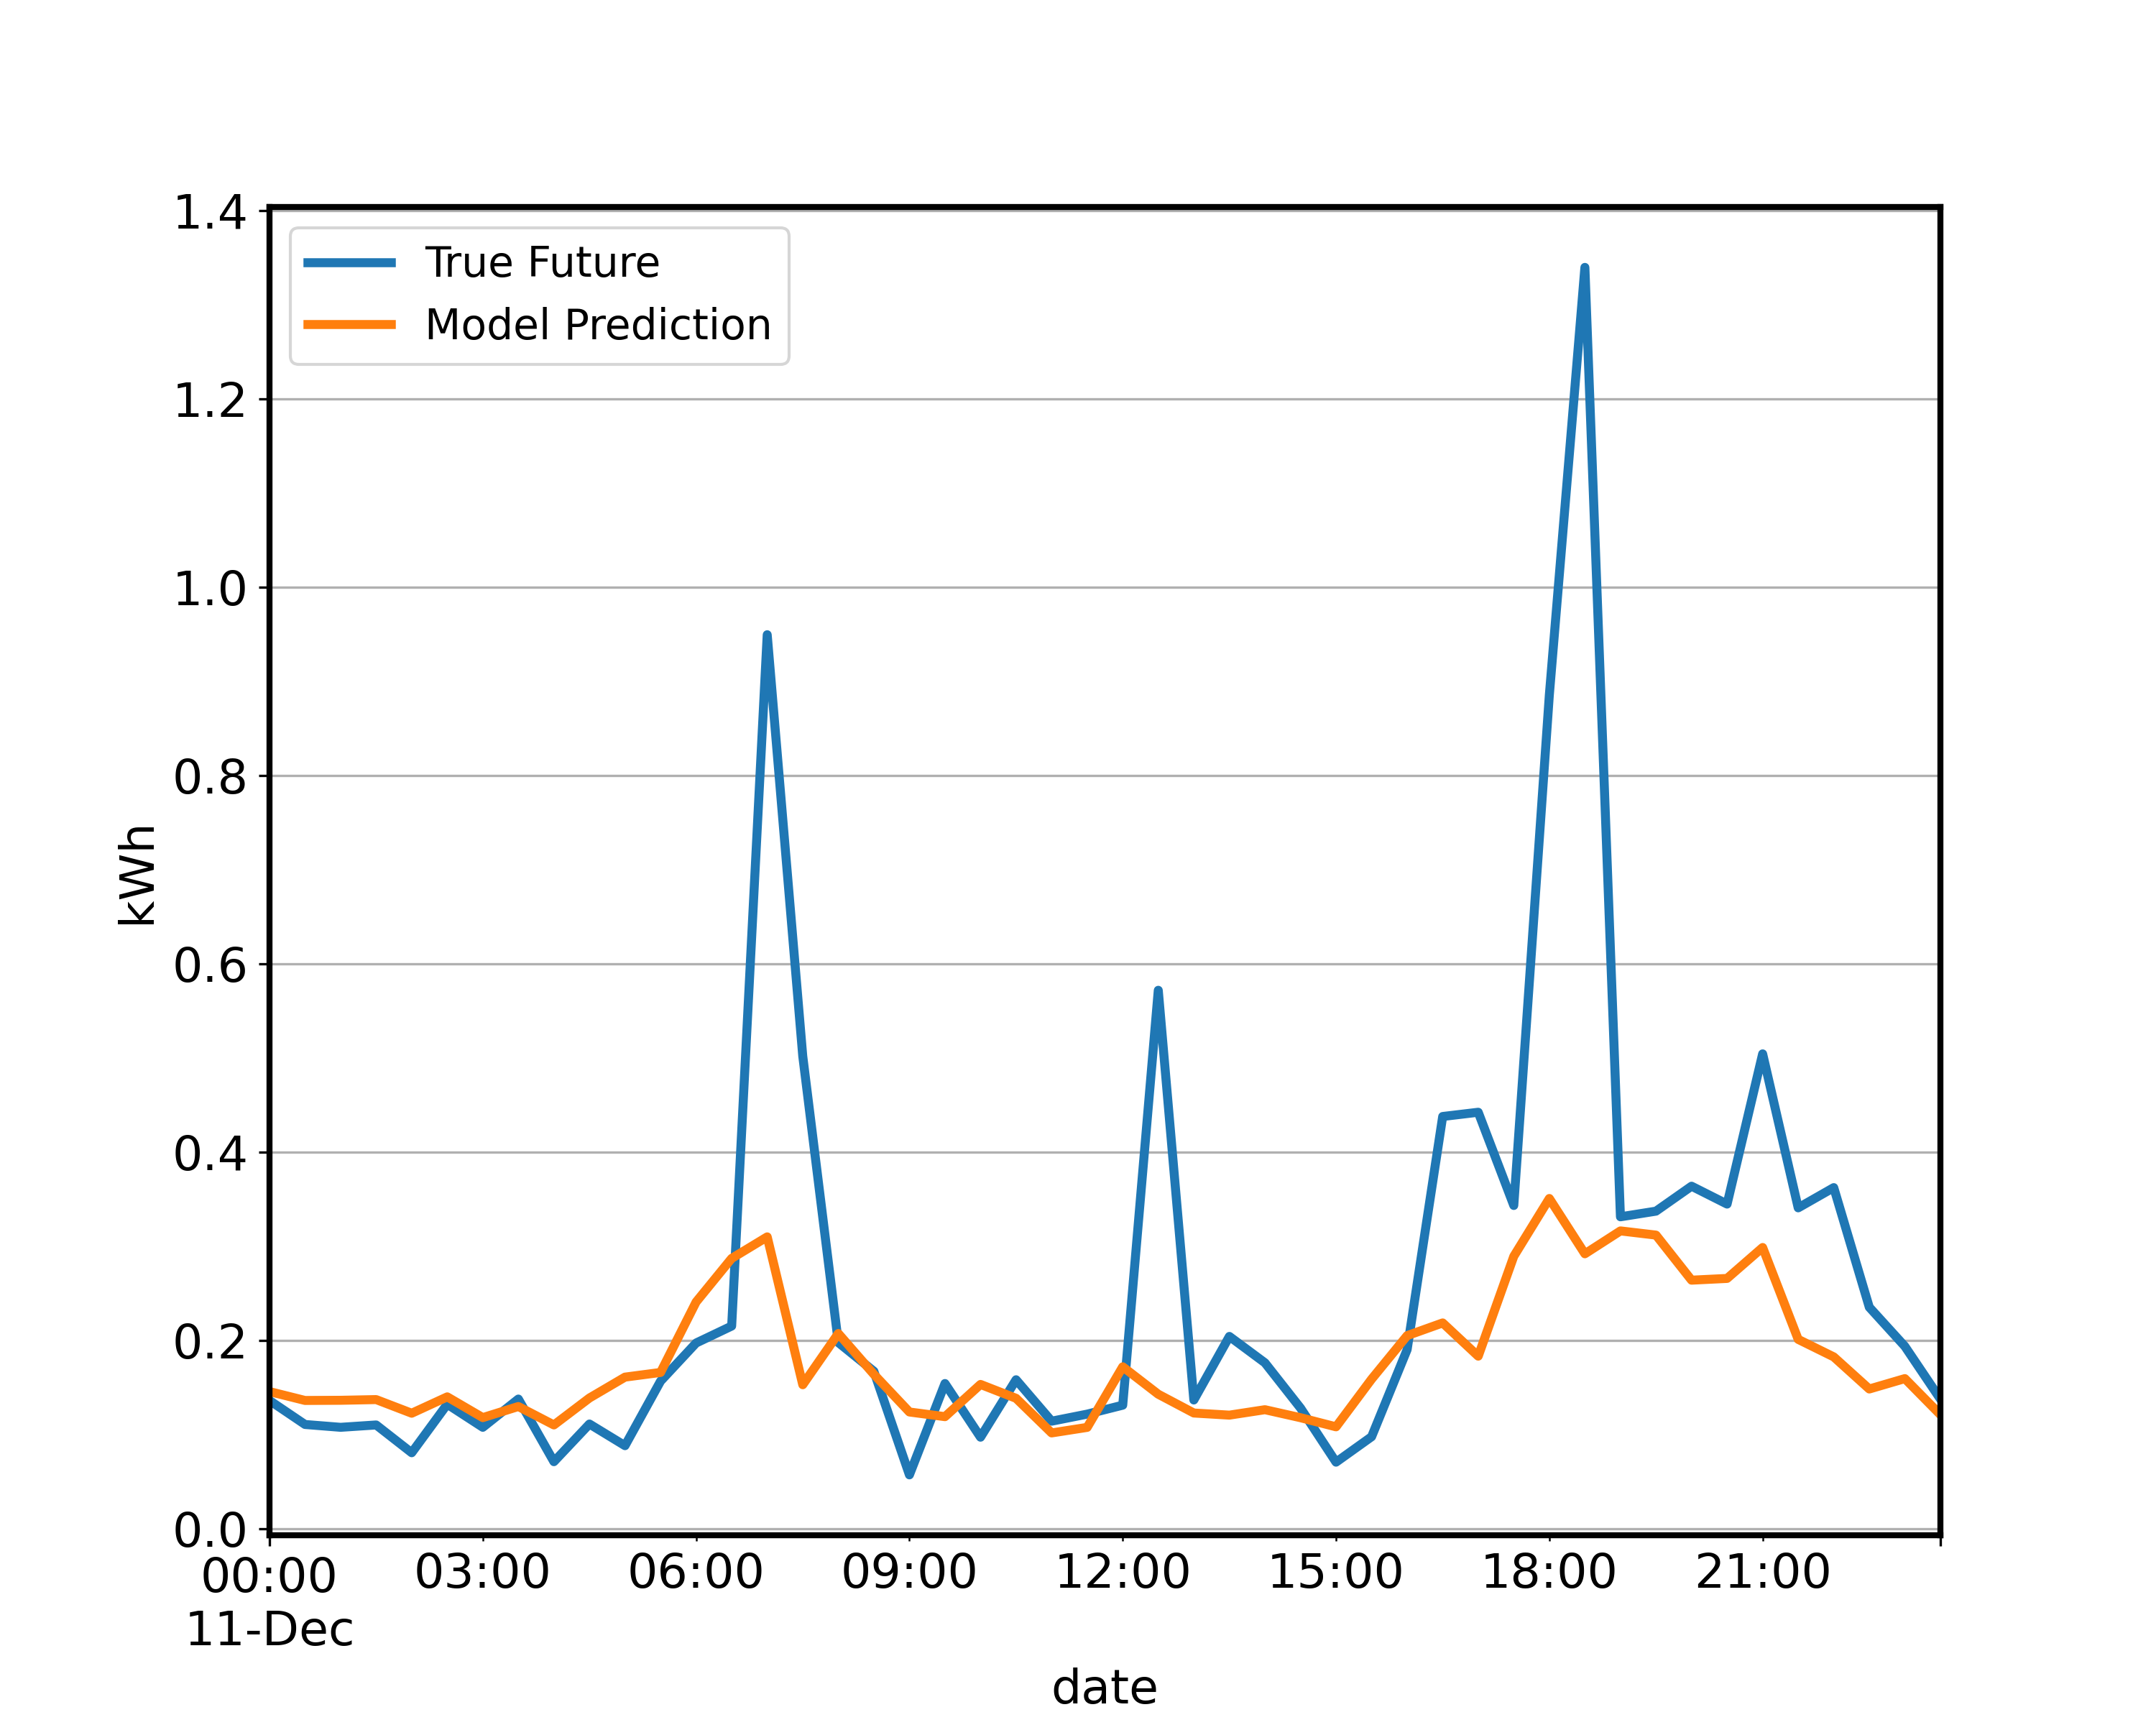
\includegraphics[width=1\linewidth]{MAPE_ID0x78a812ecd87a4b945e0d262aec41e0eb2b59fe1e_Day345_pred.png_1618425124.png}
		\caption{Model 5: ``MAPE forecast''}
	\end{subfigure}
	\caption{Daily predictions of two baseline models. (Blue: True / Orange: Prediction) }
	\label{fig:baseline models 4 and 5}
\end{figure}


Table \ref{tab:summ_data_rel_performance} shows the average performance of the baseline models on all $ 261 $ time series in the ``consumption.csv'' of Table \ref{tab:available_data} that contain a full year of measurements. The MAPE metric is not used because $ 99 $ series contain a true half hour consumption of zero, which would lead to a division by zero. The resulting error metric of every time serie is divided by the error of the model that performs worst. Then the average is taken over all the time series. The closer the averaged value is to one, the more often this model was behaving worst. By applying this normalization, the NRMSE leads to the same result as for RMSE. Therefore, only RMSE is mentioned. 

\begin{table}[ht]
	\centering
	\begin{tabular}{@{}l|ccccr@{}} \toprule
		\textbf{Error metric}	& \textbf{Closest day} & \textbf{$ 1 $ day} & \textbf{$ 7 $ days} & \textbf{mean} & \textbf{MAPE}\\\midrule
		Mean absolute error& \cellcolor{red!25}$0.950 $&$ 0.8298 $  & $0.8224 $ & \cellcolor{green!25}$ 0.7274 $ & $ 0.7918 $\\
		Mean squared error& \cellcolor{red!25}$0.8377 $&$ 0.7771 $  & $0.7363 $ & \cellcolor{green!25}$ 0.4996 $ & $ 0.6907 $\\
		Root mean square error& \cellcolor{red!25}$0.9084 $&$ 0.8621$  & $0.8426$ & \cellcolor{green!25}$ 0.6993$ & $ 0.8155$\\\bottomrule
	\end{tabular}
	\caption{Relative performance over all the $ 261 $ time series.}
	\label{tab:summ_data_rel_performance}
\end{table}

From Table \ref{tab:summ_data_rel_performance} it can again be concluded that the model performing a mean forecast attains the best results. The second best general applicable model over all the three metrics is the MAPE forecast model.

-add initialization in intro
\section{Neural network models}\label{s:Neural network models}
In this section deep LSTM models, which are models that are specialized in time series learning, are presented in different variations. The term deep is used because multiple LSTM layers are stacked on top of each other. The goal of the developed models is to make a $ 24 $ hour electrical consumption forecast for a single household. First, the general context in which the deep LSTM models are trained is explained. This covers the inputs that are feeded to the models, measures taken to avoid overfitting, the explanation of a stateless model versus a stateful model, initialization and the metrics used for evaluation. Next, the specific LSTM models developed are discussed in Section \ref{s:LSTM_implementation}. Further, follows  the discussion of the conducted parameter search in Section \ref{s:Parameter search}.

\subsection{Different practical considerations of the models in Keras}

\subsubsection{Inputs}\label{s:Inputs}
The inputs to theses models are similar as was suggested in papers \cite{loadforecastingmoor} and \cite{Kong2019}: 
\begin{itemize}
	\item historic training values (min-max normalization)
	\item average daily temperature (min-max normalization)
	\item which day of the week? (one hot encoding)
	\item which time of the day? (one hot encoding)
	\item is it a holiday? (one hot encoding)
\end{itemize}

How far will be looked back into the history of the electrical consumption is decided by the lag value. This value corresponds to the number of historic time steps that will be taken into account. The LSTM models are developed using the Keras toolbox backed by Tensorflow in Python. The Keras model expects a matrix $ \bm{X} $ as input with three dimensions: sample number, amount of time steps and amount of features. The amount of time steps equals thus the lag value. 

One sample of the $ \bm{X} $ matrix e.g. $ (1,lag\hspace{1.5mm}value, features) $, equals a 2D matix. Time steps correspond to the rows of this matrix and features to the columns. Every column contains a different time serie that serves as input. On the first column an amount of $ lag\hspace{1.5mm}value $ of previous consumption values is stored. The further down the rows of the first column, the closer time gets to the actual value that needs to be predicted. This is also the case for the temperature, but because the temperature is only known on daily basis and the history of the electricity consumption is known for every 30 minutes, the temperature value is often the same in the second column of the 2D matrix. The historic consumption and daily average temperature input are normalized by scaling between $ 0 $ and $ 1 $, using a min-max normalization.

In the next $ 7 $ columns of the 2D matrix, information is given about which day of the week it is. This is encoded making use of an one hot encoding.For every row one of the $ 7 $ columns which corresponds with the day of the week gets an one and the rest will be set to zero. Very similar the information about the time of the day is indicated. There are $ 48 $ columns and for every row only one column gets an one to indicate the time of the day. This makes that the 2D matrix has $ 59  $ columns which corresponds to the amount of features. Every 2D matrix in $ X $ serves as input to forecast a single next half hour electrical consumption.\\

When the 24 hour prediction is made, the assumption is taken that information about the real electrical consumption is known until the moment of prediction. In case of this thesis, that means until midnight the previous day. 

\subsubsection{Batch size}
A batch size has to be specified in the Keras fit function. The batch size determines how many inputs are feeded to the model and their outputs compared with their reference to define an objective function that is used when calculating the gradients for weight update. Because here only one sample is predicted per 2D input matrix, the amount of samples of $ \bm{X} $ correspond to the amount of outputs.\\

\subsubsection{Stateless versus Stateful}
Keras introduces a concept of stateless and stateful. As explained above the input given to a LSTM model is an array of data of three dimensions: sample number, amount of timesteps, amount of features. As explained in \cite{FneishMo} a stateless model interprets every sample of $ \bm{X} $, which is a 2D matrix of inputs, to contain in every column a serie that has nothing to do with the serie on the same column in a other sample of $ \bm{X} $. When processing the next sample of $ \bm{X} $, the hidden states and memory states are therefore again initialized to zero vectors. Because there is no relation between the input series over the different samples, it is logical to collect as much as possible samples for training and the input data is generated by moving a window every time one step further as can be seen in Figure \ref{fig:stateless_input}. It was found that when predictions were done also the hidden states and memory states are reset for every prediction.\\

In contrast with a stateless model, a stateful model doesn't reset its hidden states and memory states when going to the next sample in $ \bm{X} $. This means that when all the series that are contained in the separate 2D matrices are glued behind each other, the initial input signals should be recovered. How this is done can be seen in Figure \ref{fig:stateful_input} for a \textit{lag value} of three. It can however be desired to reset hidden states and memory states during training e.g. after one epoch. To achieve this, it has to be set manually. During predictions, also the hidden states and memory states are preserved. Therefore the concept of seeding before predictions becomes possible as explained in Section \ref{s:Model3}.\\

Using a stateful model introduces the additional complexity that the amount of training samples in $ \bm{X}_{training} $ and $ \bm{X}_{validation} $ should be dividable by the batch size that is chosen. This batch size then also has to be used during prediction. The circumvent these issues, a batch size of $ 1 $ is chosen for model $ 3 $ which is discussed in Section \ref{s:Model3}.\\


\begin{figure}[h]
	\centering
	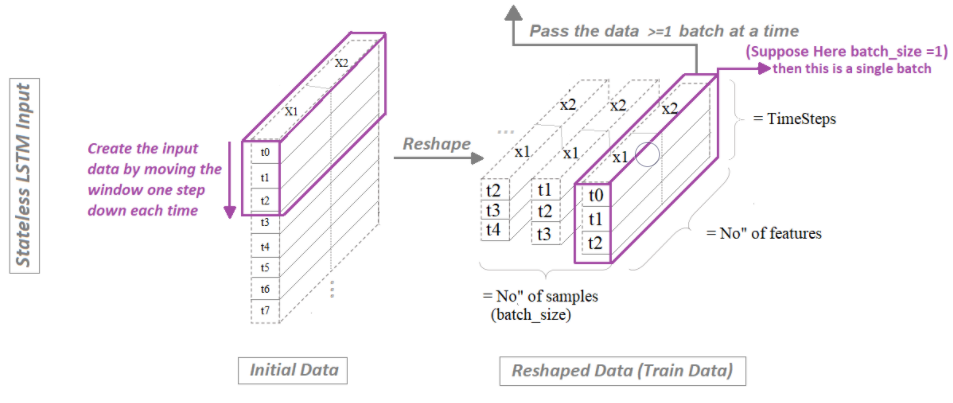
\includegraphics[width=1.2\textwidth]{stateless_input.png}
	\caption{The generation of inputs for a stateless model. (source: \cite{FneishMo})}
	\label{fig:stateless_input}
\end{figure}

\begin{figure}[h]
	\centering
	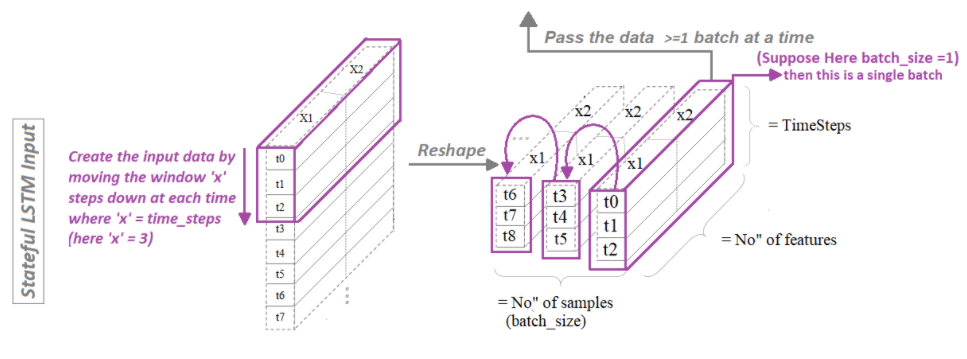
\includegraphics[width=1.2\textwidth]{stateful_input.png}
	\caption{The generation of inputs for a stateful model. (source: \cite{FneishMo})}
	\label{fig:stateful_input}
\end{figure}

\subsubsection{Initialization}
When looking at the LSTM equations in Section \ref{s:LSTM}, four weight matrices $ \bm{W} $ with an index \textit{H} and four weight matrices with an index \textit{X} can be identified. These are respectively the recurrent and kernel weights and they are both initialized in a different way. A recurrent weight matrix is initialized using a ``orthogonal'' initialization and the kernel weight matrix uses ``glorot uniform'' initialization. Both methods make use of random sampling of a distribution  during the generation of the initial values. The biases $ \bm{b} $, memory states $ \bm{c}_t $ and hidden states $ \bm{H}_t $ of the LSTM equation are all initialized by arrays filled with zeros.\\


\subsubsection{Overfitting avoidance in Keras}
Different ways to avoid overfitting can be applied in Keras and is listed as follows:
\begin{itemize}
	\item Early Stopping
	\item Dropout and recurrent dropout in the LSTM layer
	\item Dropout in the Dense layers
	\item $ l2 $ regularization on the kernel weights, recurrent weight, bias and activity.
\end{itemize}

\subsubsection{Metrics to evaluate the models}
The metrics that are used to evaluate the prediction performance of the models are the same as the ones used by the baseline models in Section \ref{s:Baseline models}:
\begin{itemize}
	\item Mean absolute error
	\item Mean squared error
	\item Normalized root mean squared error
	\item Root mean square error
	\item Mean absolute percentage error
\end{itemize}

During training also an error measure is used to accordingly update the weights of the neural network. It was found in literature that much of the time $ MSE $ is used for this.


\subsection{Deep LSTM}\label{s:LSTM_implementation}
\begin{figure}[ht]
	\centering
	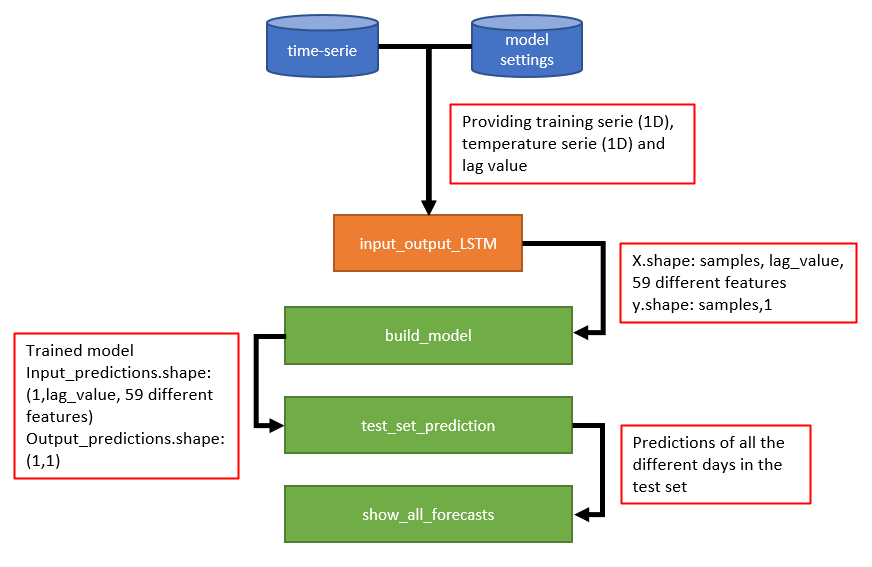
\includegraphics[width=1.2\textwidth]{flow_code.png}
	\caption{The flow of functions that are executed in order to produce daily forecasts.}
	\label{fig:model1}
\end{figure}


First, the input data of the LSTM is calculated in \textit{input\_output\_LSTM} which should be done in different ways depending on the model as is showed in Figures \ref{fig:stateless_input} and \ref{fig:stateful_input}. This is done before training by making use the GPU that is listed in Table \ref{tab:CPU}. The inputs that are used are discussed in Section \ref{s:Inputs}. \\ 
Next, the models are build. Three different models will be shown further from which the first two are stateless models and the third is a stateful model. For the stateless models it is possible to shuffle the input data. It was found that when it is desired that before splitting the inputs of the LSTM in a training and validation set the data is shuffled and not just the last part is used as validation set, shuffling should be done manually before inputted to the fit function in Keras according to Deeplizard's blog page.\\
During prediction, every model will predict only one half hour of electrical consumption at a time as was proposed as a good methodology in \cite{ANNRNN}. This concrete means that one input is feeded to the model and one output is coming out. To predict all $ 48 $ consumption values in a day, the previous predictions are used to predict consumptions later on the day. Also, each model makes use of early stopping on a validation set to avoid overfitting. The models can have multiple LSTM layers on top of each other. The hidden state vector $ \bm{H}_{j} $ serves then as input instead of $ \bm{X}_{k} $ for the layer above. The specific parameters and layout that is chosen for each of the three models is discussed in Section \ref{s:Parameter search}.

\subsubsection{Model 1: Stateless with no flatten layer}\label{s:Model1}

\begin{figure}[h]
	\centering
	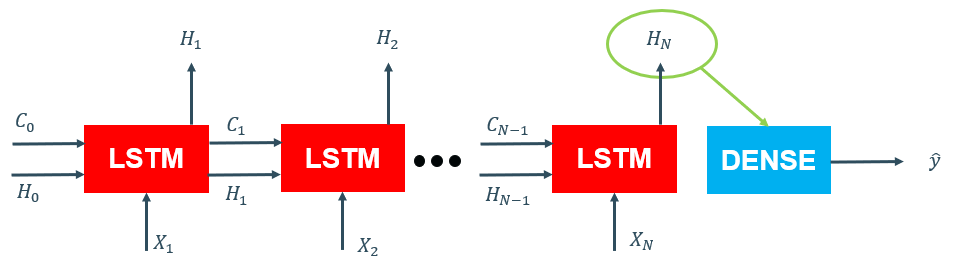
\includegraphics[width=1.2\textwidth]{model1.png}
	\caption{Model 1 - stateless model with as input a subserie of N time steps and $ \bm{C}_{i} \in \mathbb{R}^{m} $, $ \bm{H}_{j} \in \mathbb{R}^{n} $, $ \bm{X}_{k} \in \mathbb{R}^{l} $, $ \hat{y} \in \mathbb{R}^{1} $.}
	\label{fig:model1}
\end{figure}

Every subserie of the original time serie has $ N $ time steps and is feeded to the LSTM layer. When the final LSTM block is reached the output of this block will be translated to a single prediction value by a conventional layer of hidden neurons (Dense layer). The subseries are created by shifting the window one time step further in time on the original time serie. Because Model 1 is stateless $ \bm{C}_{0} $ and $ \bm{H}_{0} $ will be initialized by zero vectors. The amount of $ N $ LSTM blocks that are depicted in Figure \ref{fig:model1} equals the lag value that determines the amount of previous time steps that will be taken into account for the next prediction. Although that Figure \ref{fig:model1} gives the impression that there are multiple LSTM blocks, this only serves as a visual interpretation. There is actually only one LSTM block that is reused for every $ \bm{X}_{k} $. This means that when the same size of layers and hidden recurrent states are chosen, all the three models will have the same amount of trainable parameters. 


\subsection{Model 2: Stateless with flatten layer}\label{s:Model2}

\begin{figure}[ht]
	\centering
	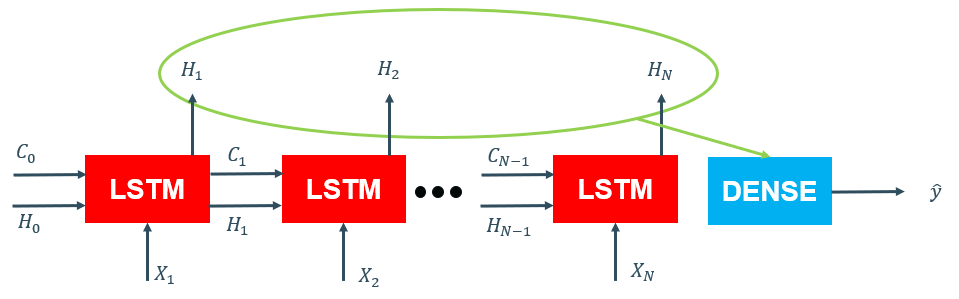
\includegraphics[width=1.2\textwidth]{model2.png}
	\caption{Model 2 - stateless model with as input a subserie of N time steps and $ \bm{C}_{i} \in \mathbb{R}^{m} $, $ \bm{H}_{j} \in \mathbb{R}^{n} $, $ \bm{X}_{k} \in \mathbb{R}^{l} $, $ \hat{y} \in \mathbb{R}^{1} $.}
	\label{fig:model2}
\end{figure}

In this model additionally to the output of the last LSTM block also the previous outputs of the LSTM blocks are inputs to the dense layer. This model corresponds to the model depicted and explained in \cite{Kong2019}.

\subsection{Model 3: Stateful}\label{s:Model3}
\begin{figure}[ht]
	\centering
	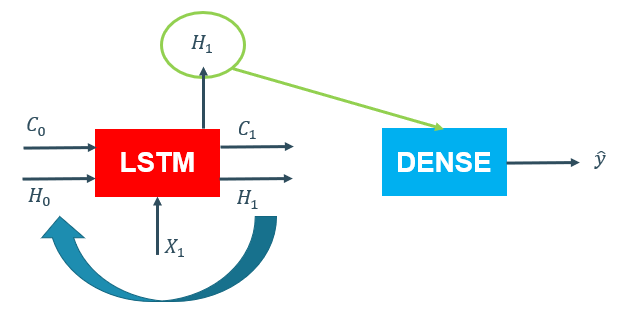
\includegraphics[width=0.8\textwidth]{model3.png}
	\caption{Model 3 - stateful model that connects single LSTM blocks and $ \bm{C}_{i} \in \mathbb{R}^{m} $, $ \bm{H}_{j} \in \mathbb{R}^{n} $, $ \bm{X}_{k} \in \mathbb{R}^{l} $, $ \hat{y} \in \mathbb{R}^{1} $.}
	\label{fig:model3}
\end{figure}

Where the previous two models only go through a small subserie of $ 48 $ or $ 96 $ time steps before making a prediction, this model sees the whole original time serie. This is possible because the model looks one by one at each sample of the original time serie e.g. $ \bm{X}_{1} $ and sets the $ C_{1} $ and $ H_{1} $ that come out as $ C_{0} $ and $ H_{0} $ when the next sample e.g. $ \bm{X}_{2}  $ of the original time serie is used. This means that the model glues every subserie of one value together, which recreates the original serie. The shape of $ \bm{X} $ is now $ (15500, 1, 59) $, which means that each sample now is not a 2D matrix but an array. After training and before prediction of the test set or validation set, it is important that the memory states $ \bm{C}_{i} $  and hidden states $ \bm{H}_{j} $ are set ``right'' for prediction of the daily consumption. Therefore, the model is first seeded which means that first all the inputs before the desired day are shown to the model. When the model then reaches the desired day, it had the chance to collect important information in the memory states and the hidden states that it can use during the prediction. A downside of using this model is that during prediction it looks only at the previous predicted electrical consumption and uses this as input to predict the next.


\subsection{Parameter search}\label{s:Parameter search}
As will be shown in this section, the different LSTM models are dependent on the choice of good parameters to be able to perform well. During a parameter search different combinations of values for the models are tried and the values that give the best results are retained. Because it is not straightforward what the influence of one parameter exactly is on the model, all the different parameters are expected to depend on each other. If all the different parameters are varied the calculation load to try all the different combinations extremely quickly increases. In order to deal with this the parameter search that is conducted is done in three stages. The cost that comes with reducing the calculation load, is that the domain of possible values is not totally searched and dependencies are neglected. During the parameter search every combination of settings is repeated three times to reduce the influence of the random initialization of the weights in the weight matrices. The error value that is used to decide if a combination of parameters behaves better or worse, is based on the average MAE on the $ 10 $ last days of November of the three runs. The $ 10 $ last days of November are thus used as validation set during the parameter search and can be used for all three models as validation set. Inspiration for the values chosen for the different parameters is based on \cite{Shi2018}.

\begin{itemize}
	\item Stage1: different model layouts are tried (calculation time $ \approx $ $ 10 $ hours)
	\item Stage 2: the most complex model is chosen and regulation is added (calculation time $ \approx $ $ 6\times4 $ hours)
	\item Stage 3: after comparing the previous model, the best is chosen and the learning rate is more precise tuned (calculation time $ \approx $ $7$ hours)
\end{itemize}

\begin{table}[ht]
	\centering
	\begin{tabular}{@{}l|r@{}} \toprule
		\textbf{Parameter}	& \textbf{Values}\\\midrule
		Hidden states &  $ [20,50] $\\
		LSTM layers & $ [1,3] $\\
		Neurons dense layer & $ [50] $\\
		Dense layers & $ [1] $\\
		Lag value & $ [48,96] $\\
		Number epochs & $ [2] $\\
		Batch size & $ [48] $\\
		Learning rates & $[ 10^{-4} $,$ 10^{-3} $,$ 10^{-2} ]$\\
		Shuffle & $ [True] $\\
		Repeat & $ [3] $\\\bottomrule
	\end{tabular}
	\caption{Parameters used during phase 1 for the two stateless models.}
	\label{tab:para_phase1}
\end{table}

The different values of the parameters that are used can be seen in Table \ref{tab:para_phase1}. A total of $ 24 $ combinations are tried and each combination was run $ 3 $ times. The batch size chosen is only one number to make a fair comparison between the different setting with respect to the amount of weight updates that will be performed. With a batch size of $ 48 $, there are around $ \frac{15500}{48}\approx 320 $ weight updates per epoch and $ 640 $ in total. One LSTM layer is compared with three LSTM layers on top of each other in order to catch a clear difference in the influence of the amount of layers used. Because only two epochs are considered to reduce the calculation load during the parameter search, no early stopping is used during the parameter search.\\

Minor changes to the parameters in Table \ref{tab:para_phase1} are made for model $ 3 $. In model $ 3 $ a batch size, a lag value of one and shuffling ``False'' are used. A batch size of one is chosen because then the prerequisite for a stateful model is fulfilled that the training set and validation set must be divisible by the batch size and more importantly, that the batch size during training equals the one during prediction. To avoid these issues, it was first experimented with using a batch size during training that was bigger than one and then rebuilding the model with a batch size of one. The latter model would then be used during prediction. The trained weights of the first model where transferred to the second model. However, after testing it was found that the \textit{get\_weights()} and \textit{set\_weights()} commands in Keras didn't reproduce the same prediction results when used on different models. It could only be used on the same model to set the weights to the ones a chosen amount of epochs back during training. This is useful e.g. during the manual implementation of early stopping to restore the weights that performed best. Setting the weights on different models is however possible in the underlying tensorflow package, but not in Keras. In this thesis, it was chosen to solve the batch size issues for a stateful model by setting the batch size equal to one.\\

In phase two, the assumption is made that a more complex model will be able to better capture the non-linear relations in the data and regulation is added to avoid overfitting behaviour. The learning rate that was part of combination of parameter values that performed best during phase one, is selected together with the lag value. During phase two the amount of hidden states is taken equal to $ 50 $ and the amount of LSTM layers to $ 3 $. The regulation that is shown in Table \ref{tab:regulation}, is always added one at a time. The synergy between different regularization methods is thus neglected. 

\begin{table}[ht]
	\centering
	\begin{tabular}{@{}l|r@{}} \toprule
		\textbf{Kind of regularization} & 	\textbf{Kind of dropout}\\\midrule
		regularizer on input weight matrix LSTM 	& dropout inputs LSTM\\\hline
		regularizer on recurrent weight matrix LSTM & dropout recurrent states\\\hline
		regularizer on DENSE layer & dropout dense layer\\\hline
		$[ 10^{-2} $,$ 10^{-3} $,$ 10^{-4}$, $ 10^{-5} ]$ & $[ 0.2 $,$ 0.3 $,$ 0.4$, $ 0.5 ]$\\\bottomrule
\end{tabular}
\caption{Different regularization added during phase 2.}
\label{tab:regulation}
\end{table}


When l2-norm regularization is added to a weight matrix, the size of the weight using the l2-norm is added in the objective function. This means that big weight values are seen as an artificial error and the model tries to keep the weights small. The regularization parameter defines the ratio between the model focussing on the error with the reference signal and the size of the weights. Setting a big regularization parameter will give a model that becomes less ``expressive''. Therefore, the regularization parameter will contribute in the avoidance of overfitting.\\ 
The dropout layer that is used after the LSTM layer and after the Dense layer sets a rate of its inputs to zero. Similar, the dropout and recurrent dropout parameters in the LSTM layer drop respectively a rate of its inputs $ \bm{X}_{k} $ and $ \bm{H}_{j} $ to zero. The dropout rate values that are chosen are chosen between $ 0.2 $ and $ 0.5 $ as is advised in \cite{Mele1993}.\\

As will be further shown and as was found in \cite{Greff2017}, the learning rate is a very important parameter that has to be tuned correctly to enhance the model performance. Therefore a bigger range of learning rates is tried for the model that performed best after stage one and two of the parameter search. Afterwards, the learning rate which leads to the the smallest error is selected. The different learning rates that are tried are $ 10^{-2} $, $ 5\times10^{-3} $, $ 2\times10^{-3} $, $ 10^{-3} $, $ 10^{-4} $ and $ 10^{-5} $. \\

In order to speed up the calculations, multithreading is implemented to calculate separate runs in different threads. It was found that one thread takes considerably longer than when the full CPU is used to calculate the same run, but still a time gain is obtained in a total of $ 4 $ runs.\\

The importance of setting good parameters is stressed by the fact that for certain parameters the loss during training becomes ``not a number''. This is because the model becomes unstable and gets a very big loss which eventually becomes a nan. When this occurs the model is tried again with different initialization of the weights, which often solves the problem or a nan value is included as error. 


\subsubsection{Model 1: Stateless with no flatten layer}

\textbf{Phase1:}\\
Table \ref{tab:relative_performance_parameters_phase_one_model_one} shows the parameter search using the parameters listed in Table \ref{tab:para_phase1}. The search was ran on a local machine (see Table \ref{tab:CPU}) for $ 9 $ hours and $ 48 $ minutes. It is clear from Table \ref{tab:relative_performance_parameters_phase_one_model_one} that when the learning rate is varied this has the most impact on the average performance of the model. This result corresponds with paper \cite{Greff2017} where it was concluded that this parameter is the most important when tuning a LSTM. Next, it can be seen that the lag value of $ 96 $ time steps didn't lead to much more improvement with respect to looking at $ 48 $ historic time steps during every prediction. A reason for this can be that the day, two days ago, is not very representative for the desired day. It can be argued that the desired day a week ago would add more value, because this better captures the human weekly routine. In comparison Model $ 3 $ traverses the whole historic signal before making predictions. It is therefore expected that that model better captures the weekly routine.\\
An unexpected result that was found is that less LSTM units and only one LSTM layer in the case of Serie 1 gives raise to a lower MAE. The reason for this could be the presence of overfitting when using a more complex model. Table \ref{tab:best_performing_para_phase1} gives the combination of settings that performed best during phase one. In the next phase of the parameter search, regulation is added and compared with the results obtained during phase one of the parameter search. \\

\begin{table}[ht]
	\centering
	\begin{tabular}{@{}l||c|ccc@{}} \toprule
		\multicolumn{5}{c}{Model 1: Stateless (no flatten layer)}\\\midrule\midrule
		\textbf{Chosen parameter}	& \textbf{Value} & \textbf{Serie $ 1 $} & \textbf{Serie $ 2 $} & \textbf{Serie $ 3 $}\\\midrule
		Units LSTM & $ 20 $ & $12.08 $		&$ 1.24 $  & $1.48 $\\
		 		   & $ 50 $ & 		  		&		   & 		\\\hline
		layers LSTM & $ 1 $ & $9.82 $		&		   & 		\\
				    & $ 3 $ & 	      		&$ 4.26 $  & $5.80$\\\hline
		Lag value & $ 48 $ & $4.25 $ 		&		   & $0.390$\\
				  & $ 96 $ &          		&$ 2.06 $  & 		\\\hline
		Learning rate & $ 10^{-2} $ &       &		   & 		\\
					& $  10^{-3} $ &$0.0594 $&$ 17.2$  & $10.6$\\
					& $  10^{-4} $ &$8.74 $&$ 25.0$    & $12.2$\\\bottomrule
			
	\end{tabular}
	\caption{Each value in this table shows the average error when the value of a chosen parameter was used, normalized by the biggest error of the possible values and finally subtracted by one. Therefore, each value shows a percentage of improvement with respect to the worst possible value for a chosen parameter for each serie during phase $ 1 $ of the parameter search. For example: when $ 20 $ LSTM units are chosen, this on average gave a $ 12.08\% $ lower MAE.}
	\label{tab:relative_performance_parameters_phase_one_model_one}
\end{table}


\begin{table}[ht]
	\centering
	\begin{tabular}{@{}l|ccc@{}} \toprule
		\multicolumn{4}{c}{Model 1: Stateless (no flatten layer)}\\\midrule\midrule
		\textbf{Parameters}	& \textbf{Serie $ 1 $} & \textbf{Serie $ 2 $} & \textbf{Serie $ 3 $}\\\midrule
		Units LSTM & $20 $&$ 50 $  & $20 $\\
		layers LSTM & $1 $&$ 3 $  & $3$\\
		Lag value & $96 $&$ 96$  & $48$\\
		Learning rate & $0.01 $&$ 0.0001$  & $0.0001$\\\hline
		MAE error 1   & $ 0.133 $ & $ 0.0426 $ & $ 0.100 $\\
		MAE error 2   & $ 0.135 $ & $ 0.0433 $ & $ 0.100 $\\
		MAE error 3   & $ 0.138 $ & $ 0.0428 $ & $ 0.101 $\\\bottomrule
	\end{tabular}
	\caption{The values of the parameters that performed best for the three time series during phase $ 1 $ using model $ 1 $ based on the smallest sum of MAE errors during three runs.}
	\label{tab:best_performing_para_phase1}
\end{table}


\textbf{Phase 2}\\
In this section the learning rate and the lag value of the best performing model are combined with the most complex model with regulation. With most complex model, it is meant that $ 50 $ LSTM units and $ 3 $ LSTM layers are used. A sensitivity analysis is done to look which regulation has the most effect. Finally, the results of phase two are compared with the best results of phase one. Note, that using this approach assumes that adding regulation can nullify the use of a too complex model. When LSTM regularization is added this done the same on each LSTM layer.


\begin{figure}[h!]
	\centering
	\begin{subfigure}{0.49\linewidth}
		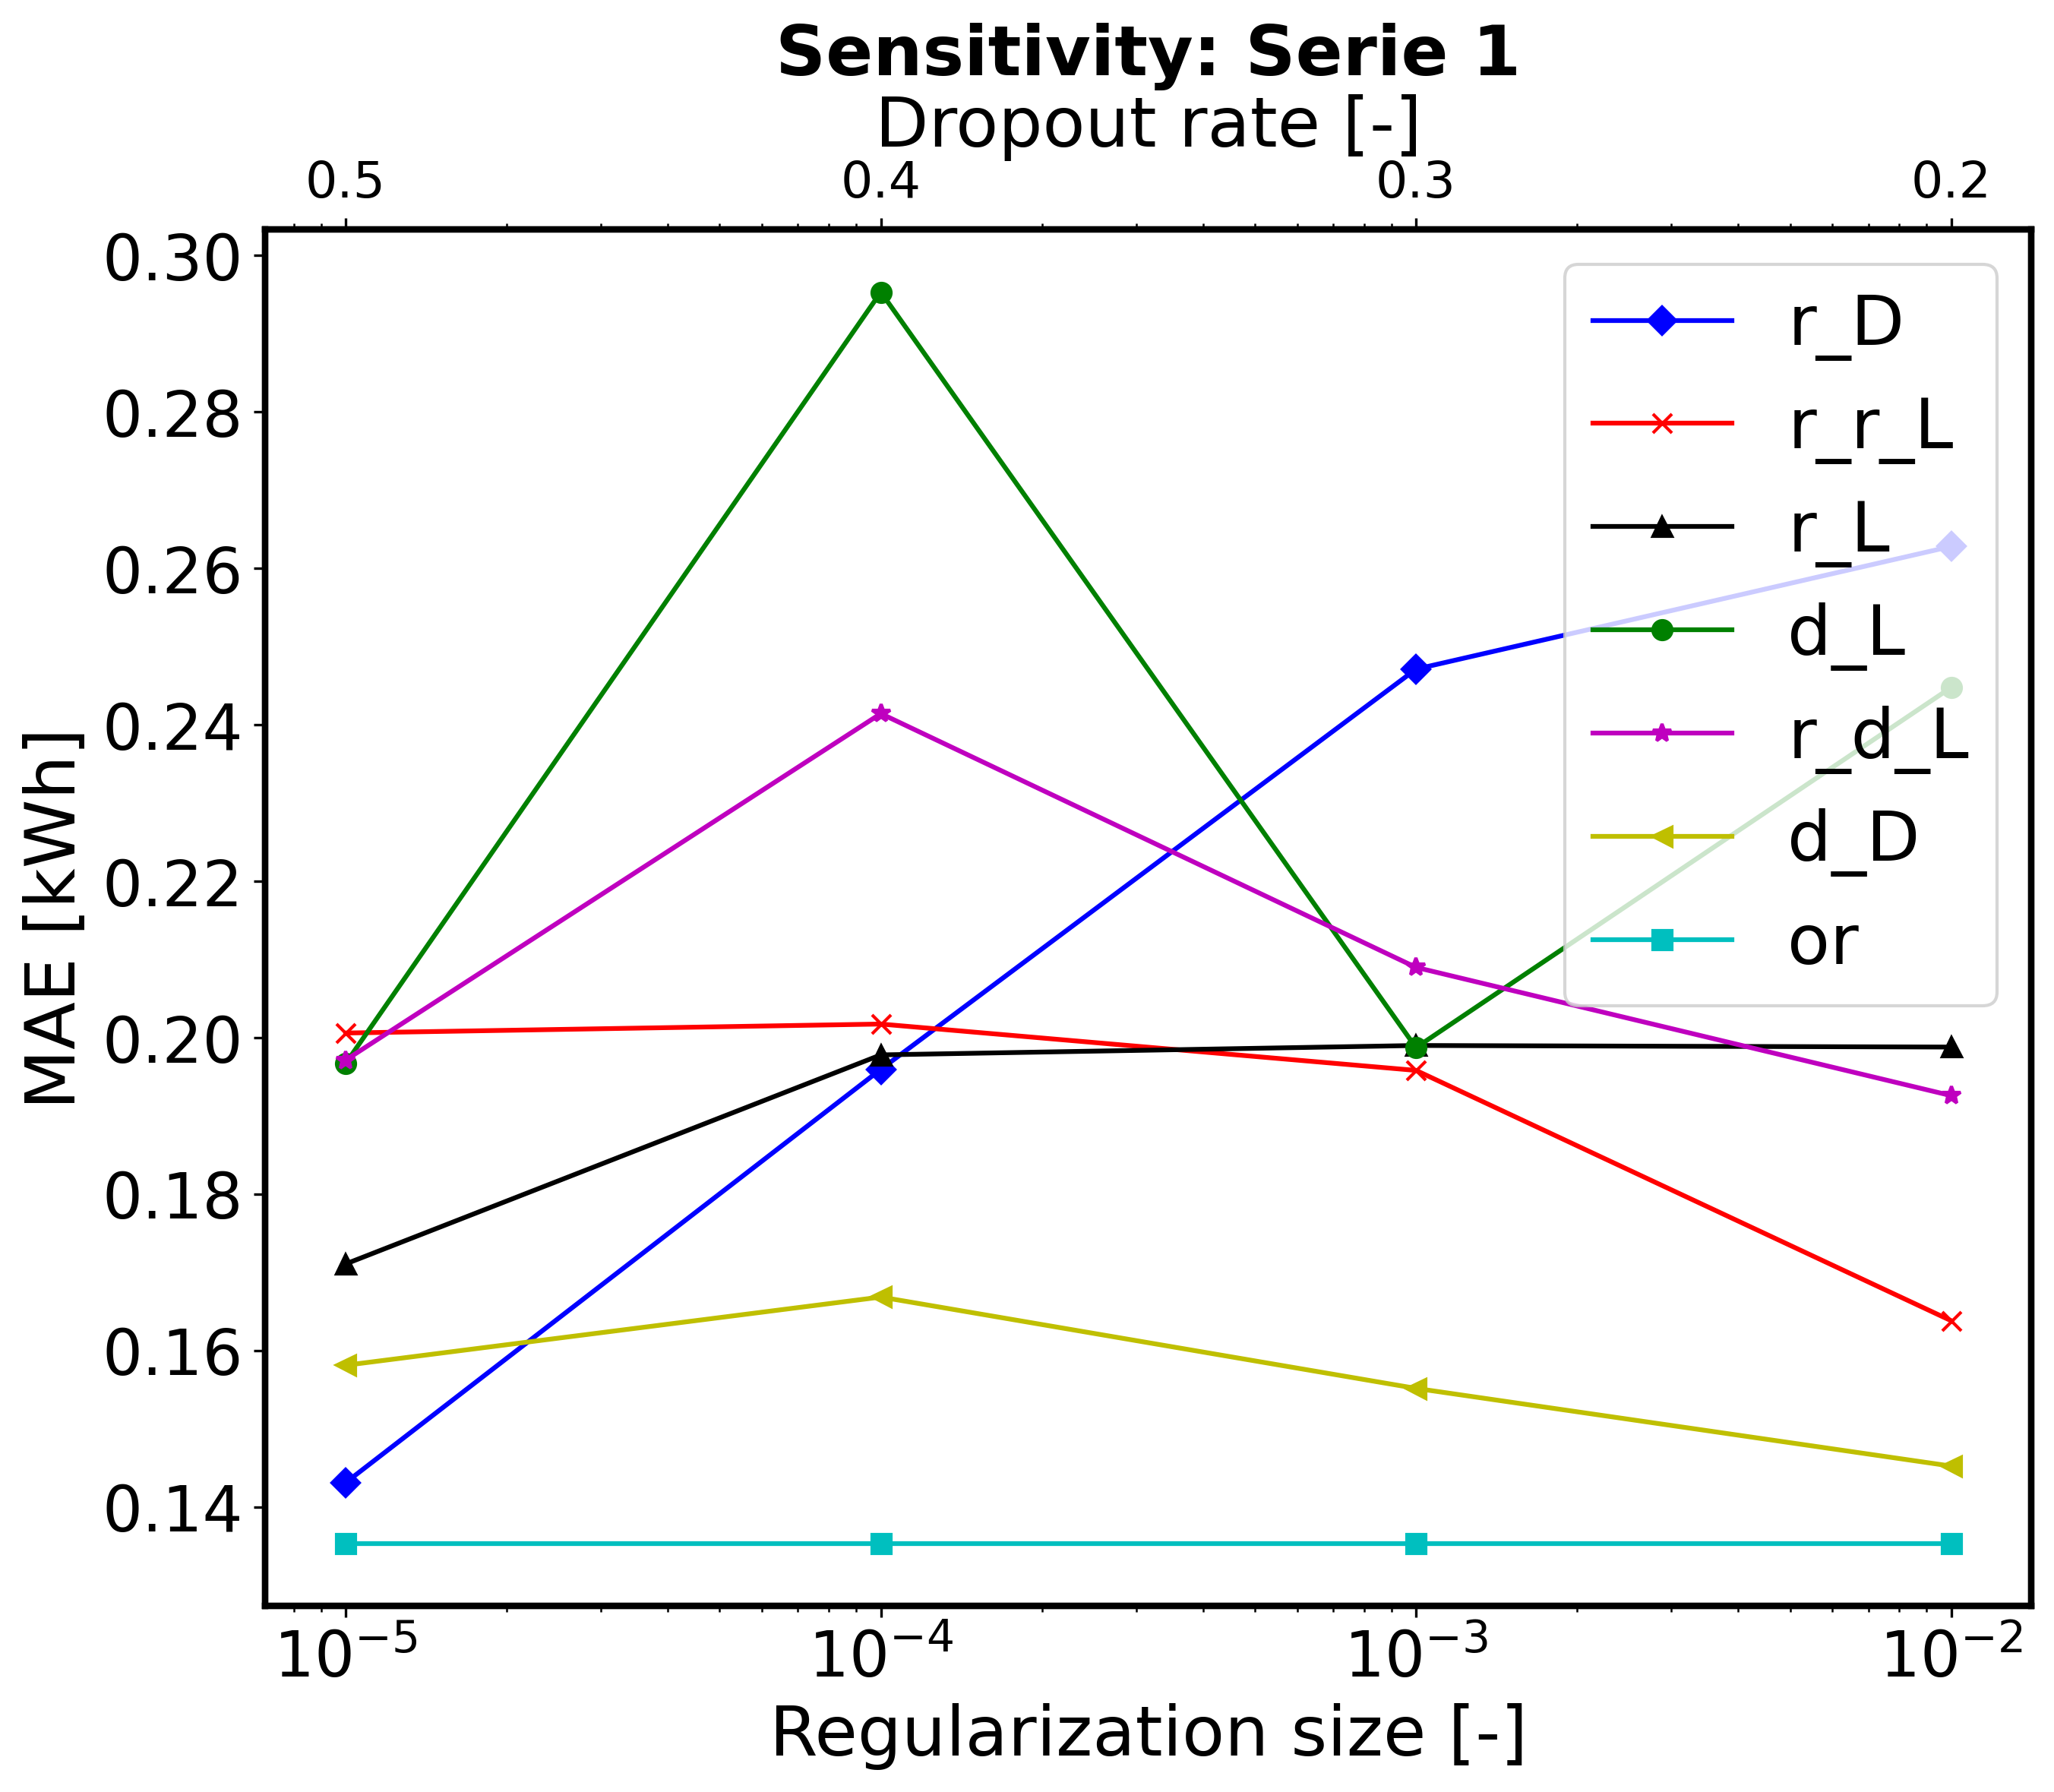
\includegraphics[width=1\linewidth]{serie1_model1.png}
		\caption{Model 1}
	\end{subfigure}	
	\begin{subfigure}{0.49\linewidth}
		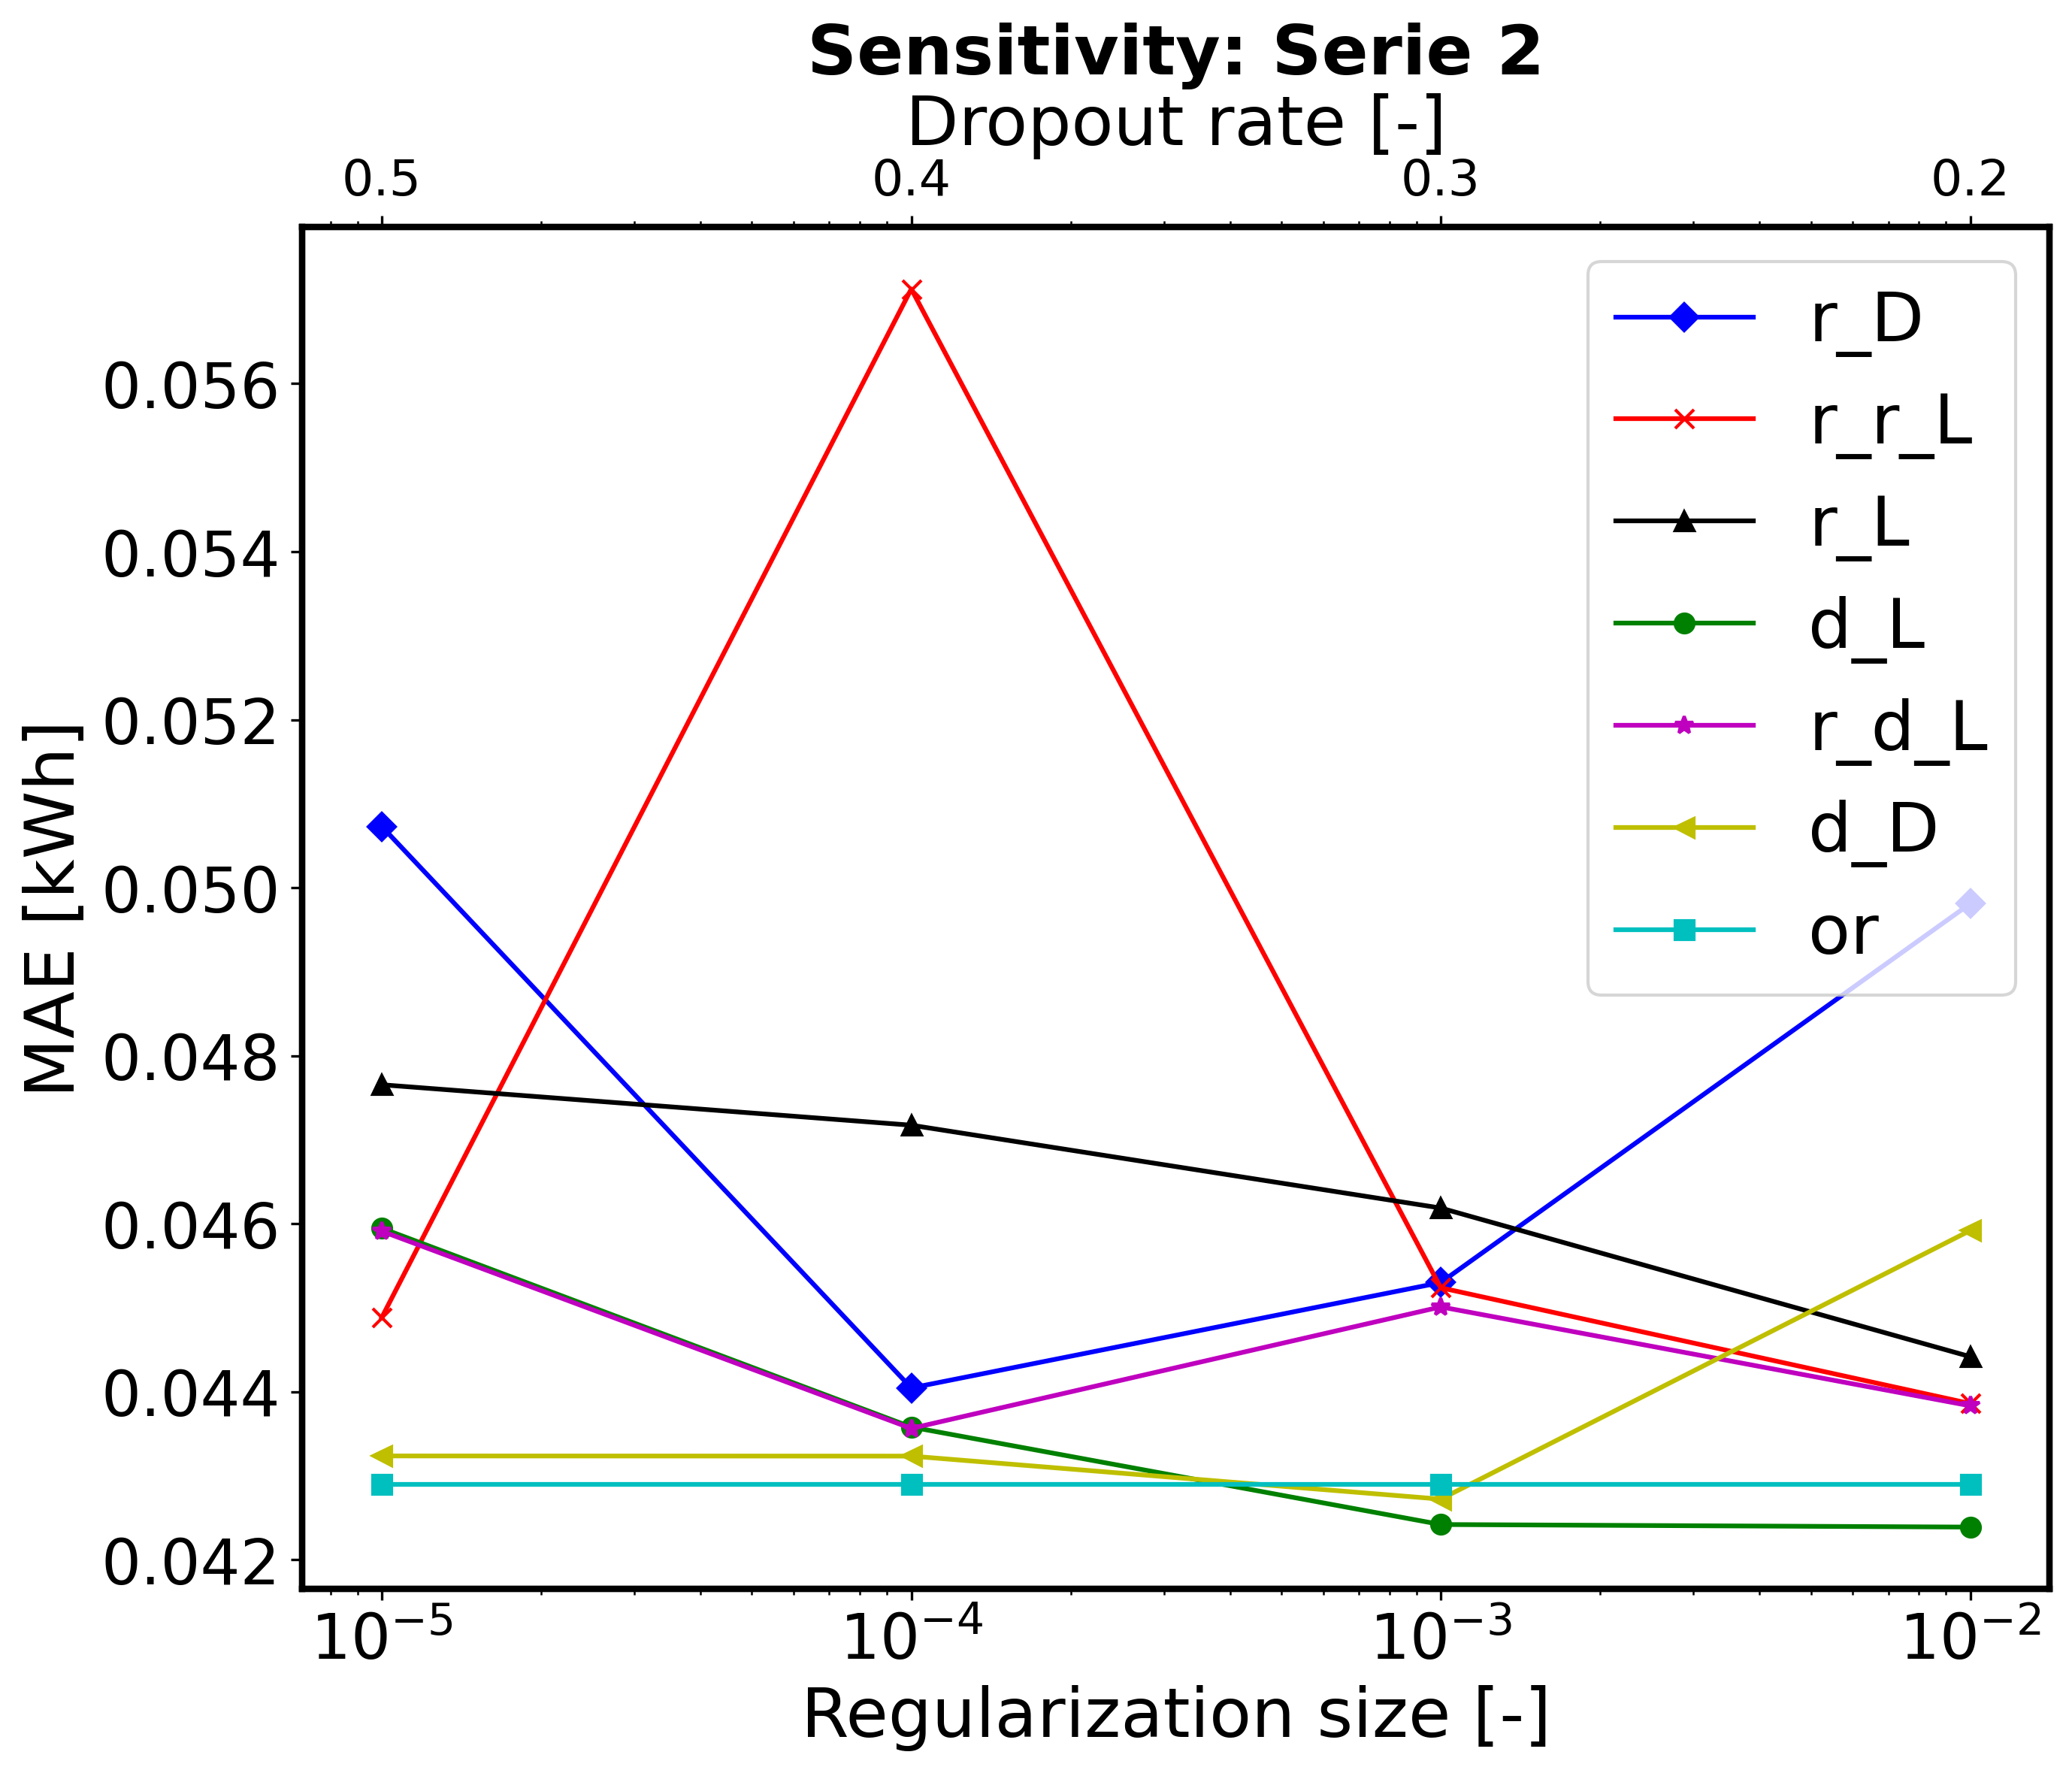
\includegraphics[width=1\linewidth]{serie2_model1.png}
		\caption{Model 1}
	\end{subfigure}
\begin{subfigure}{0.5\linewidth}
	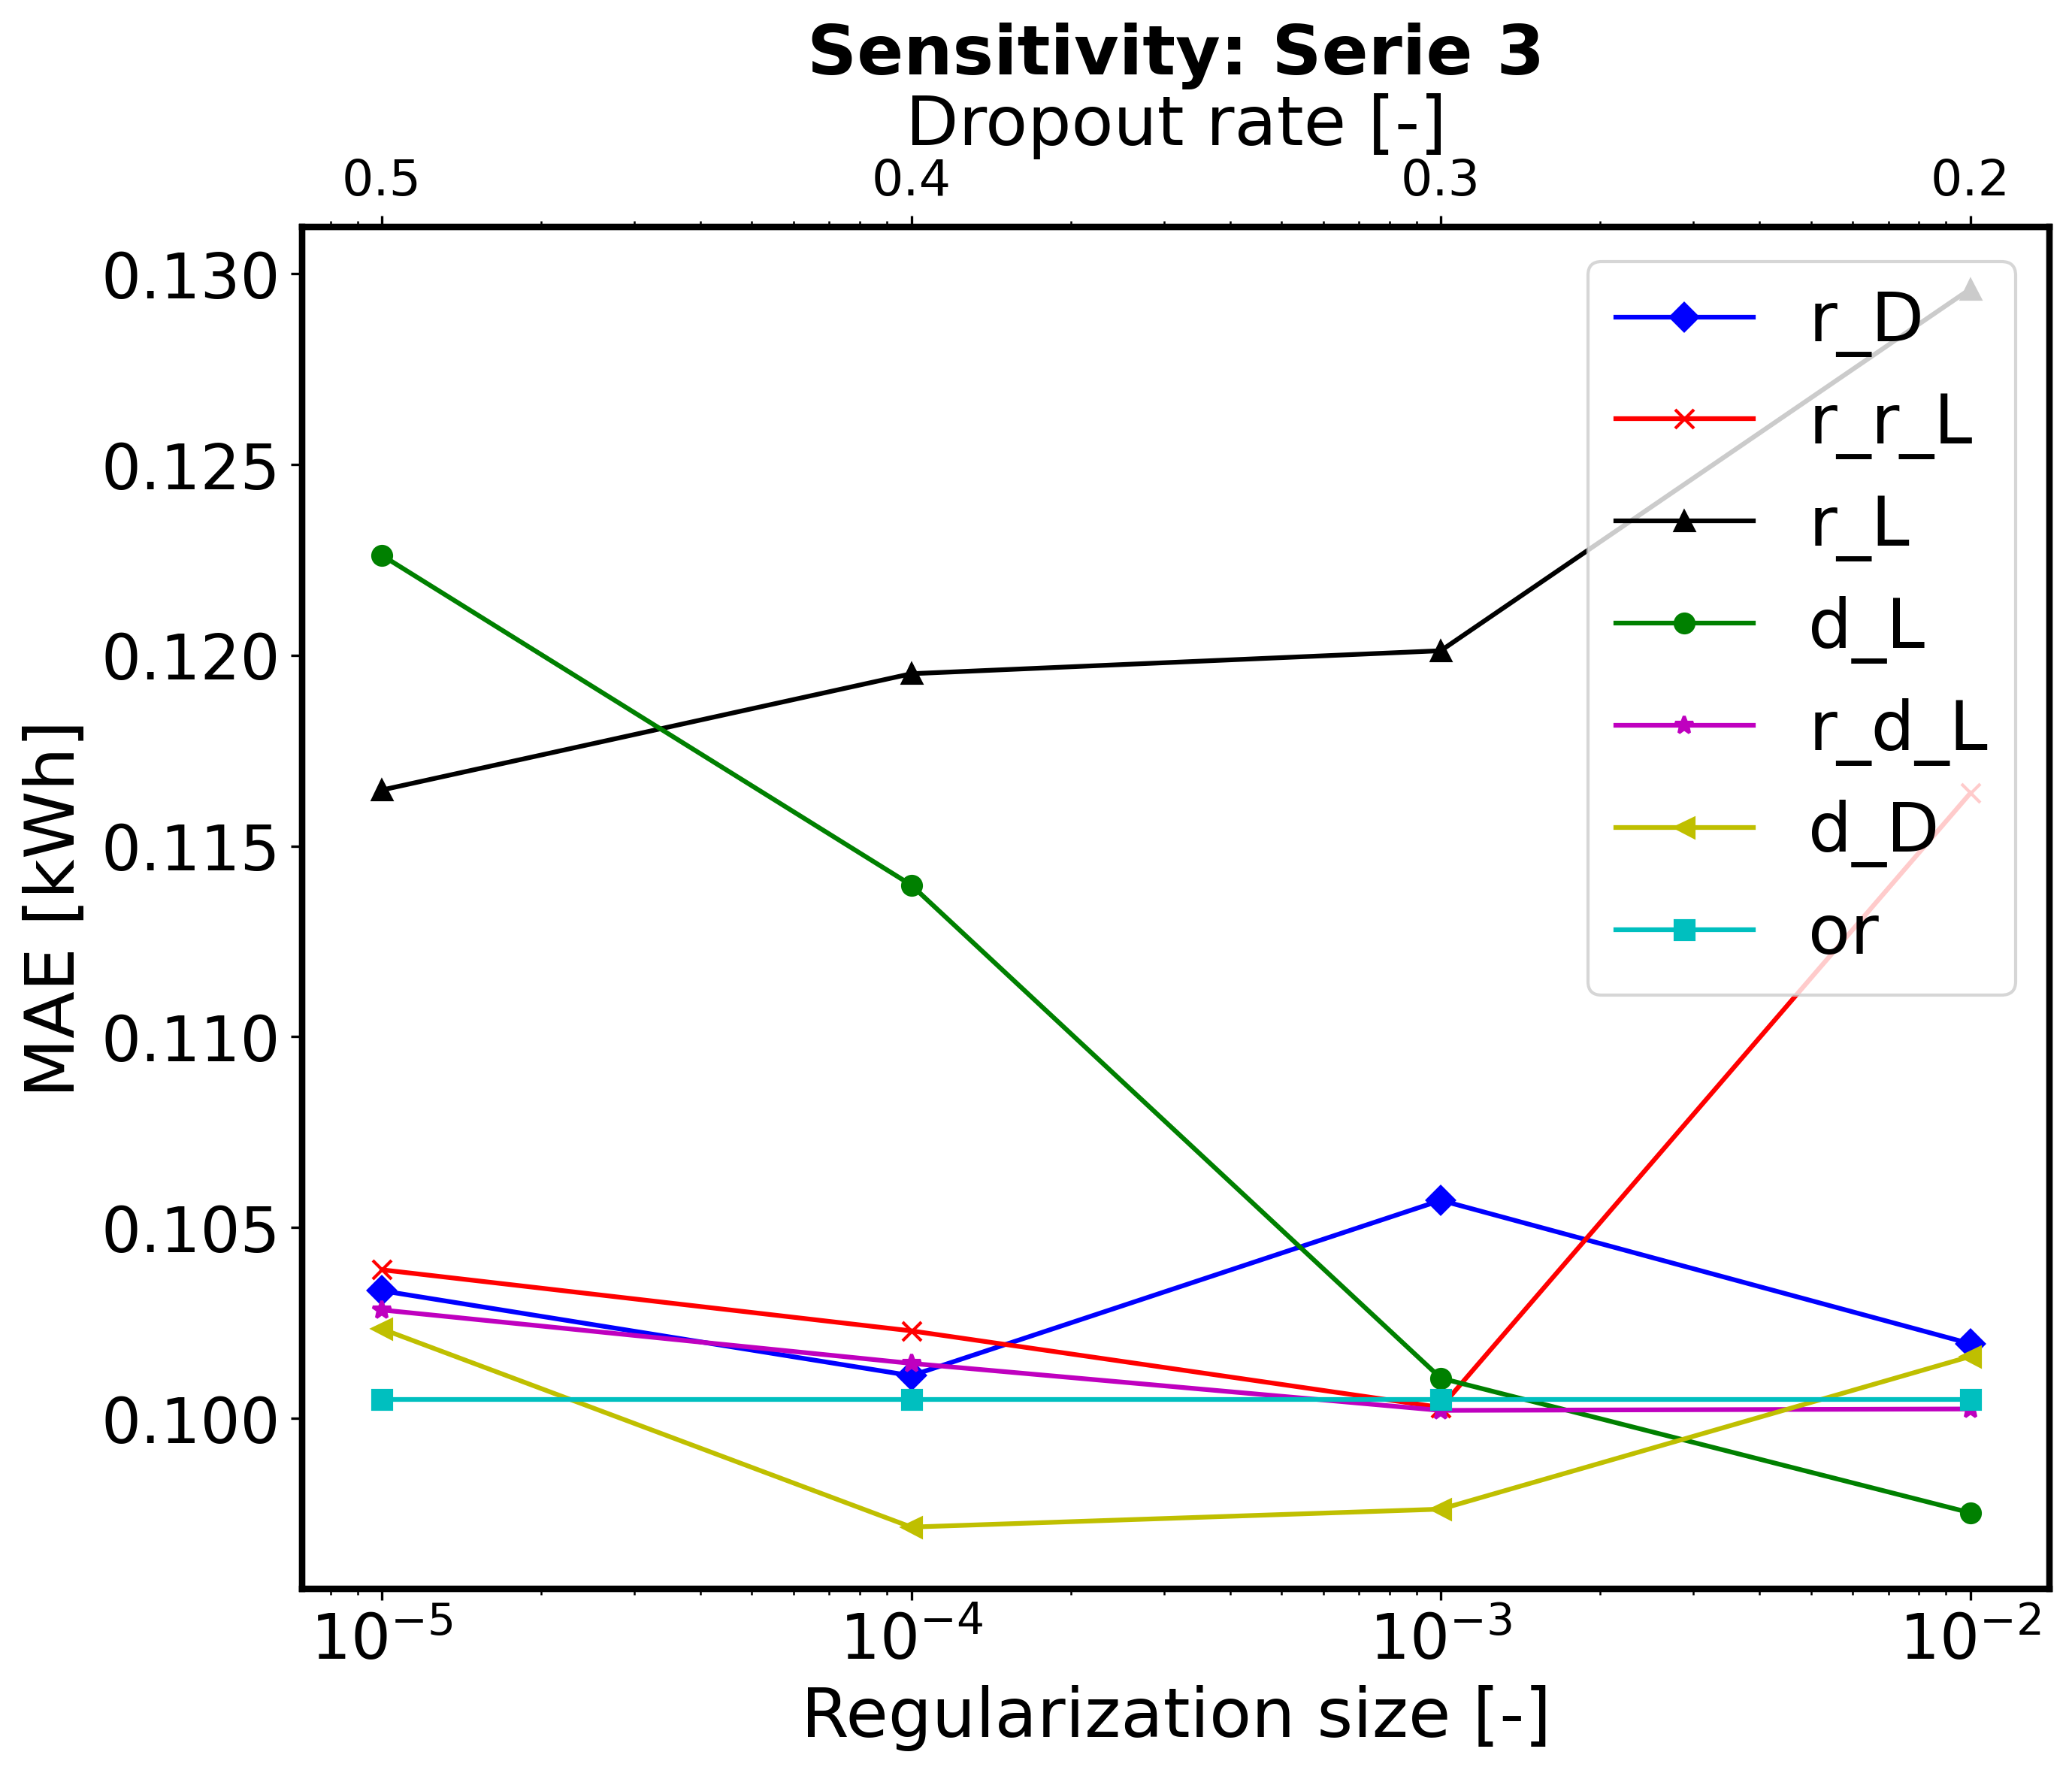
\includegraphics[width=1\linewidth]{serie3_model1.png}
	\caption{Model 1}
\end{subfigure}
	\caption{Results of the sensitivity analysis on the size of regulation parameter and the dropout rate with respect to the mean absolute error.(Legend: \textit{r\_D}: regularization size of weights DENSE layer,  \textit{r\_r\_L}: regularization size of recurrent weight of LSTM, \textit{r\_L}: regularization size of input weights of LSTM, \textit{d\_L}: dropout rate of input states LSTM, \textit{r\_d\_L}: dropout rate of recurrent states LSTM, \textit{d\_D}: dropout rate of DENSE layer, \textit{or}: best performing serie from phase one)}
	\label{fig:sensitivity_model1}
\end{figure}

From Figure \ref{fig:sensitivity_model1} it follows that:
\begin{itemize}
	\item Serie 1: The best setting during phase one as shown in Table \ref{tab:best_performing_para_phase1} outperformed all settings during phase two. 
	\item Serie 2: The best setting after phase one and two is when a dropout rate of $ 0.2 $ is added on the input states of the LSTM together with $ 3 $ LSTM layers and $ 50 $ hidden states.
	\item Serie 3: The best setting after phase one and two is when a dropout rate of $ 0.4 $ is added on the dense layer together with $ 3 $ LSTM layers and $ 50 $ hidden states.
\end{itemize}


\textbf{Phase 3}\\
Finally, during this phase special attention is devoted to the learning rate. As was displayed in Table \ref{tab:relative_performance_parameters_phase_one_model_one} changing the learning rate could lead to significant differences in model performance. Therefore, a sensitivity analysis is performed and the best learning rate is chosen for the best model after phase one and two of the parameter search. Figure \ref{fig:learning_rate_model1} shows as expected a U-shape error in function of the learning rate. A learning rate that is chosen too large is vulnerable to oscillations and will not convergence and a learning rate that is too small will take a very long time to attain good results and therefore have an increased error when compared on a fixed amount of epochs. The resulting U-shape corresponds to what is found in \cite{Greff2017} .\\

\begin{figure}[h]
	\centering
	\begin{subfigure}{0.49\linewidth}
		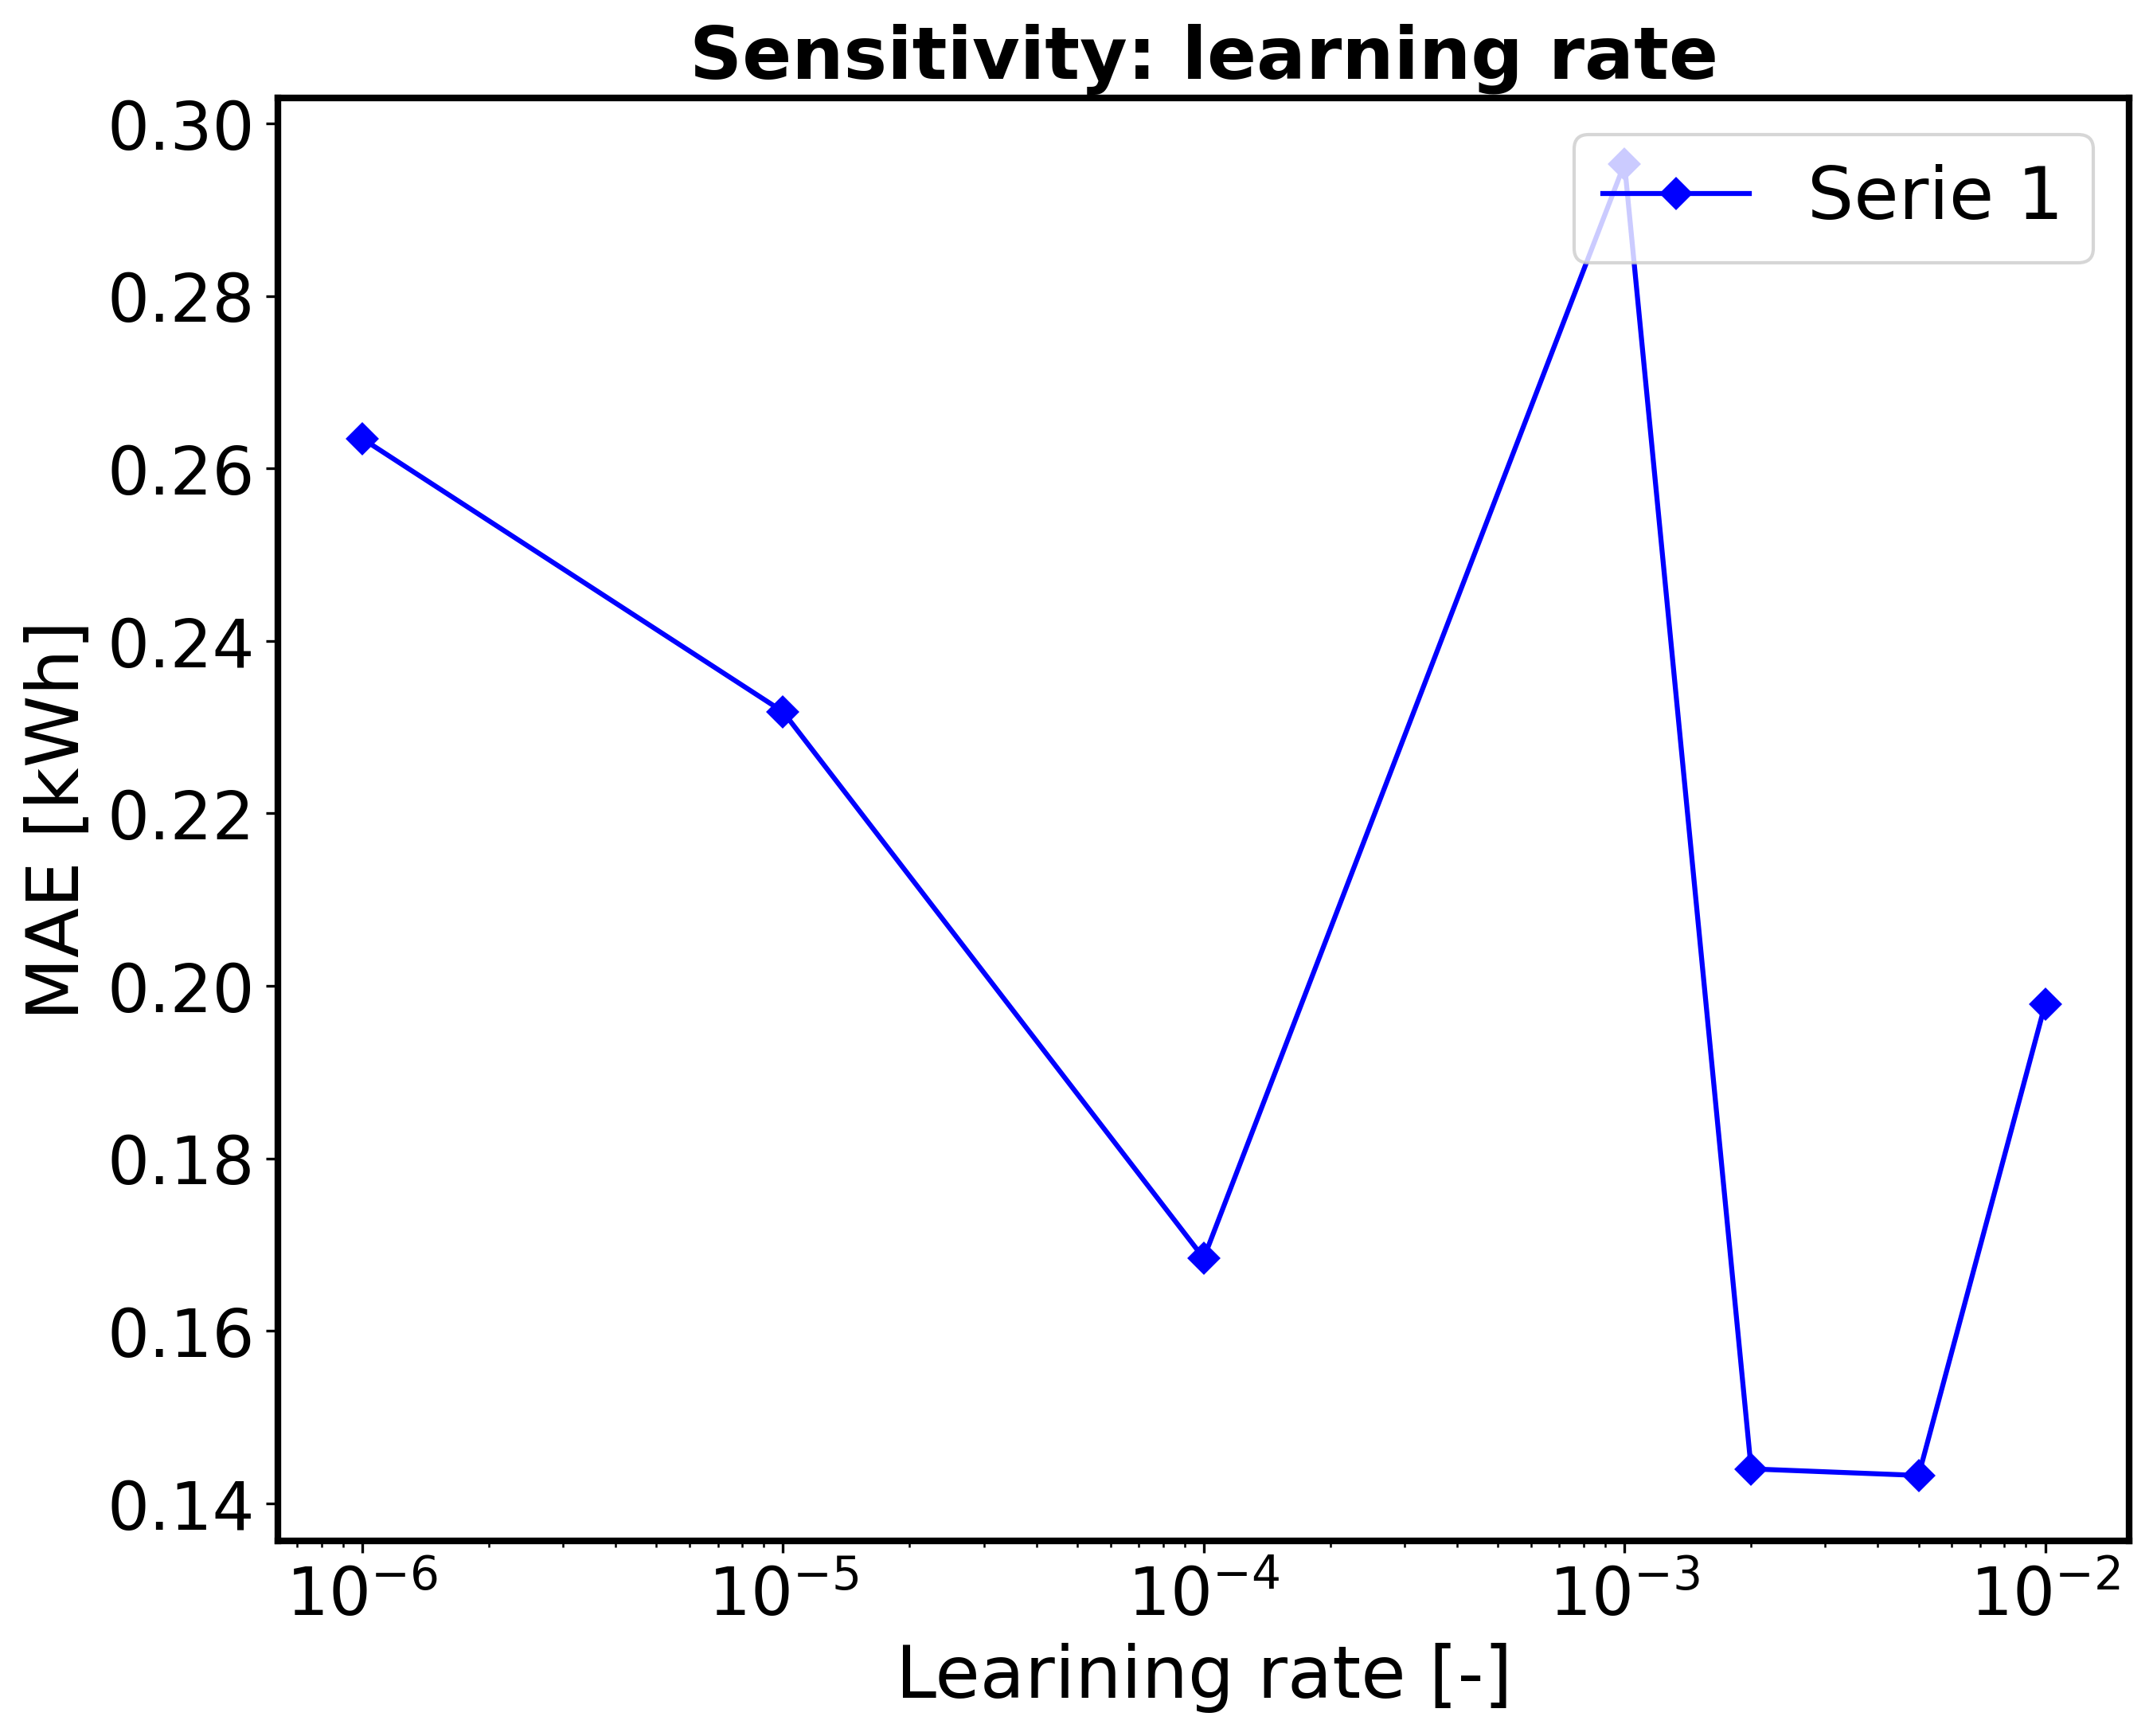
\includegraphics[width=1\linewidth]{learning_rate_serie1_model1.png}
		\caption{Model 1}
	\end{subfigure}	
	\begin{subfigure}{0.49\linewidth}
		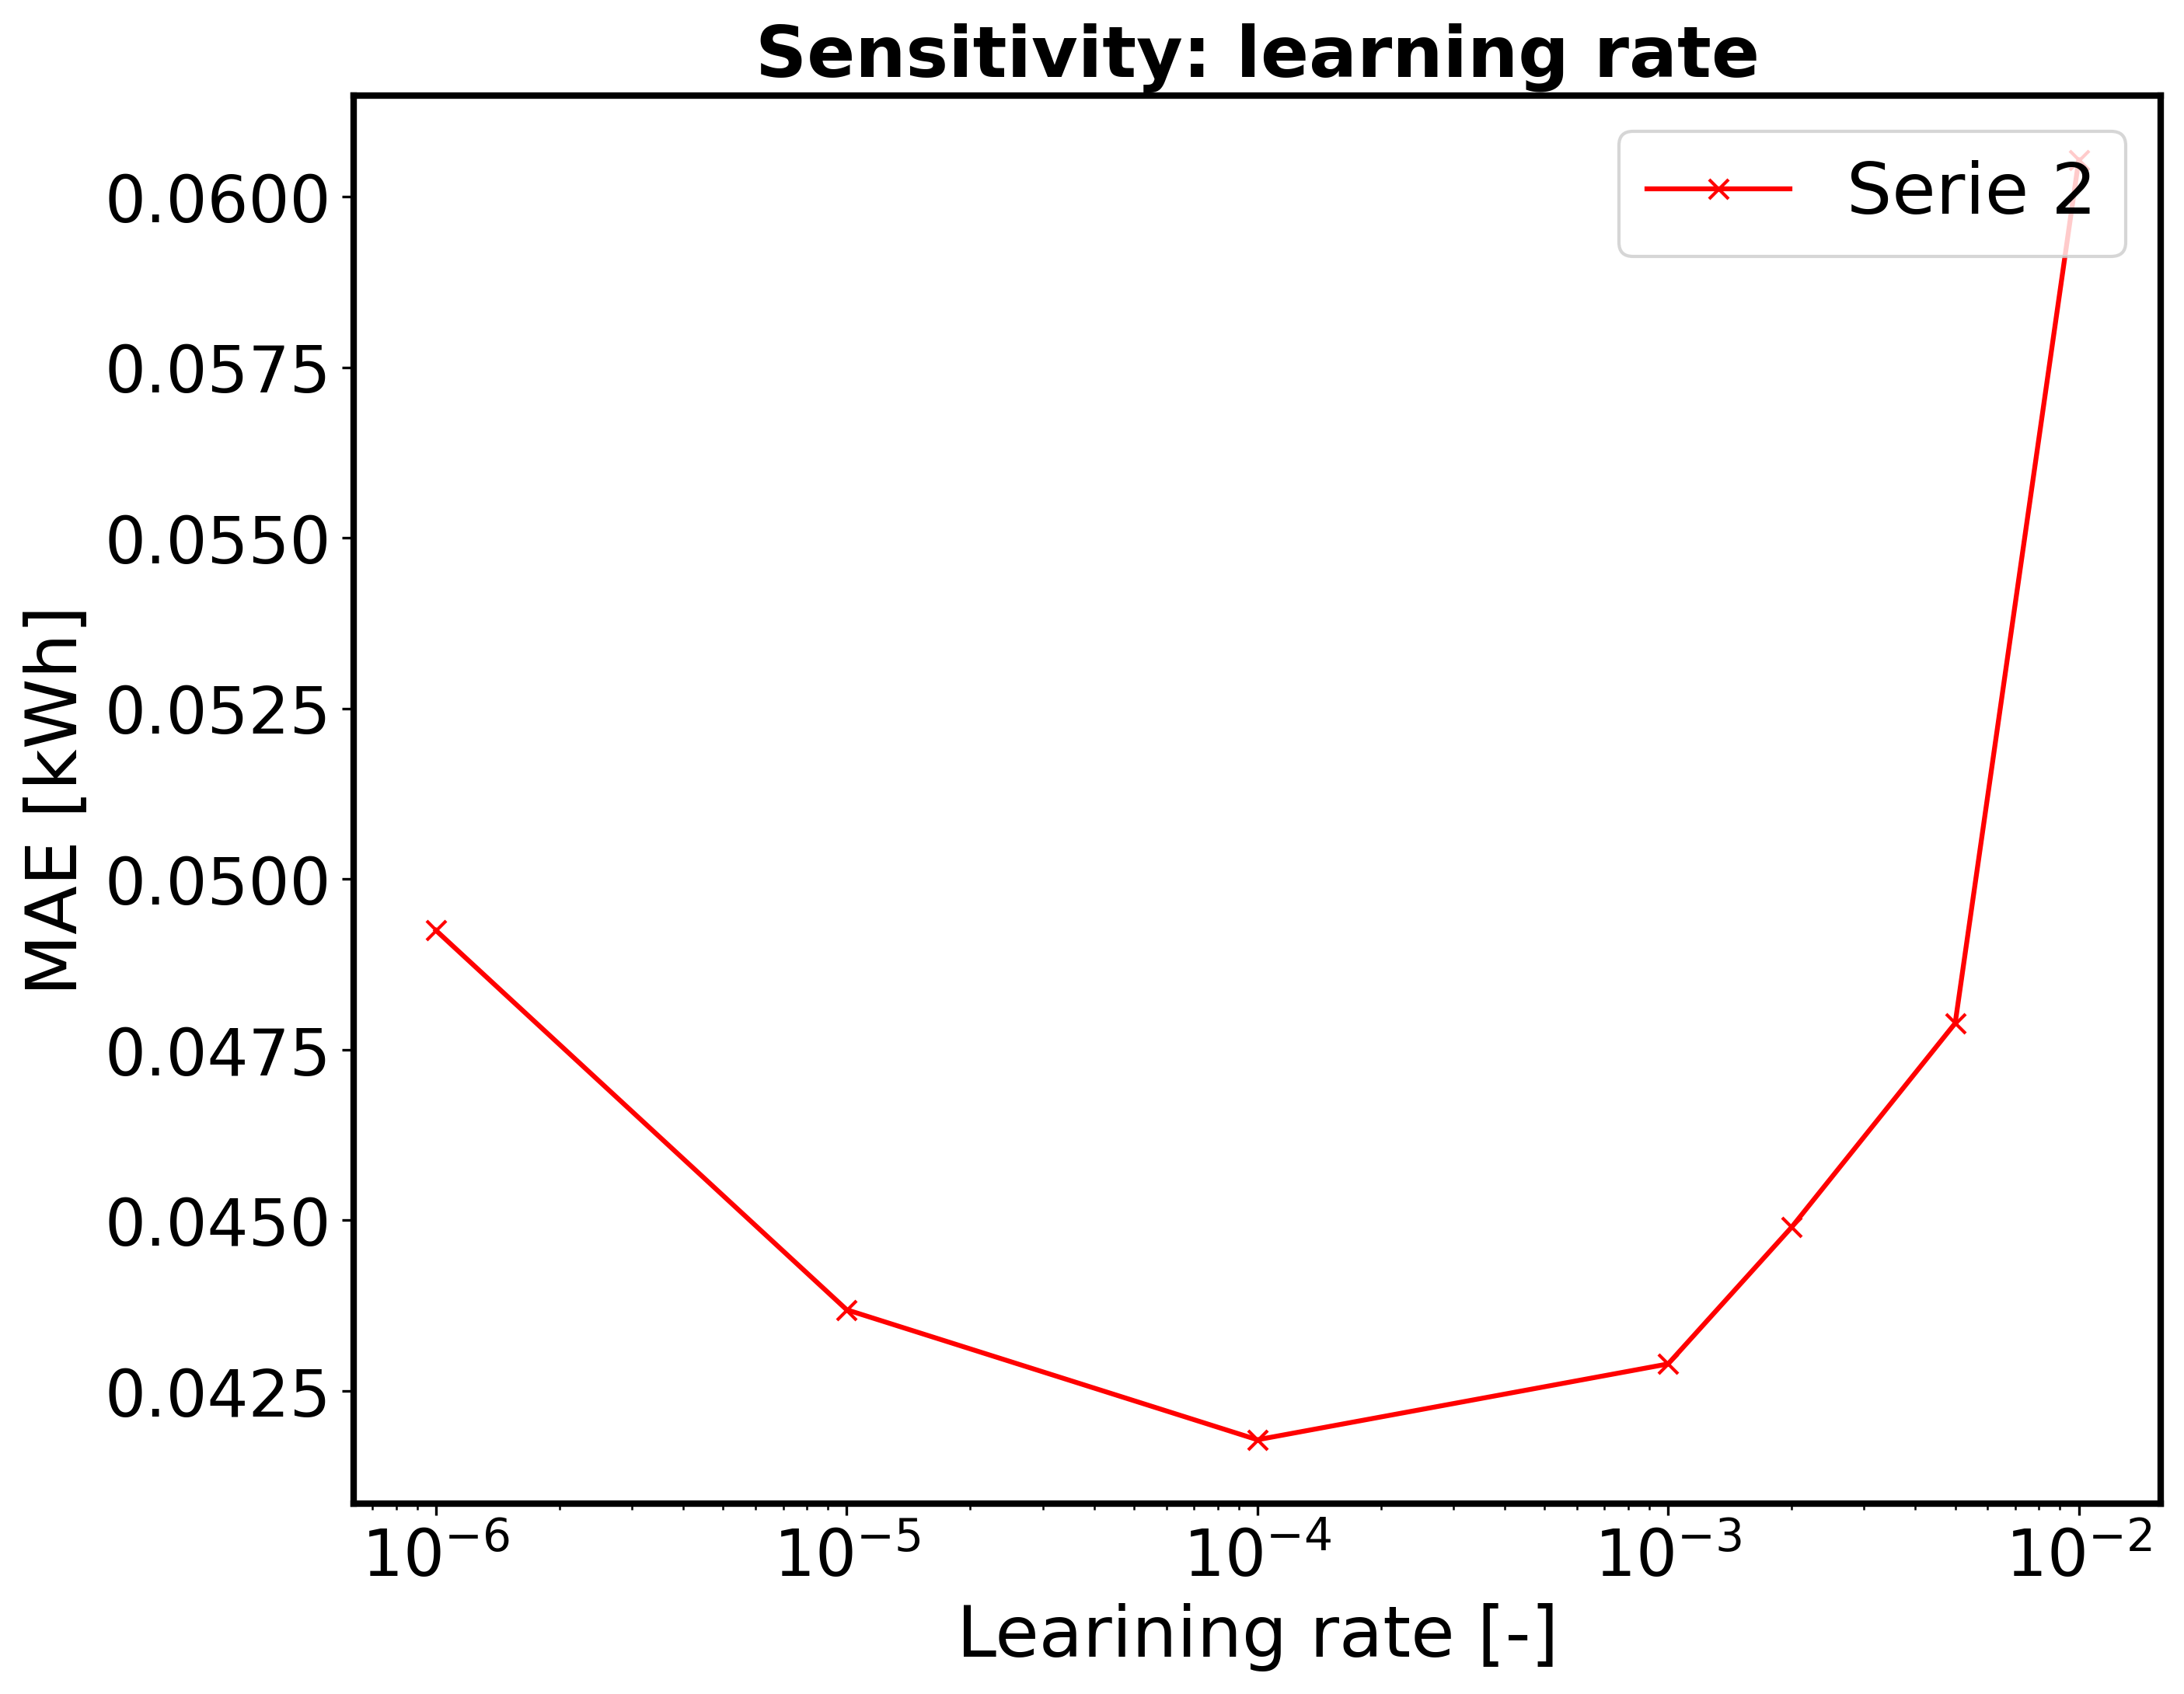
\includegraphics[width=1\linewidth]{learning_rate_serie2_model1.png}
		\caption{Model 1}
	\end{subfigure}
	\begin{subfigure}{0.5\linewidth}
		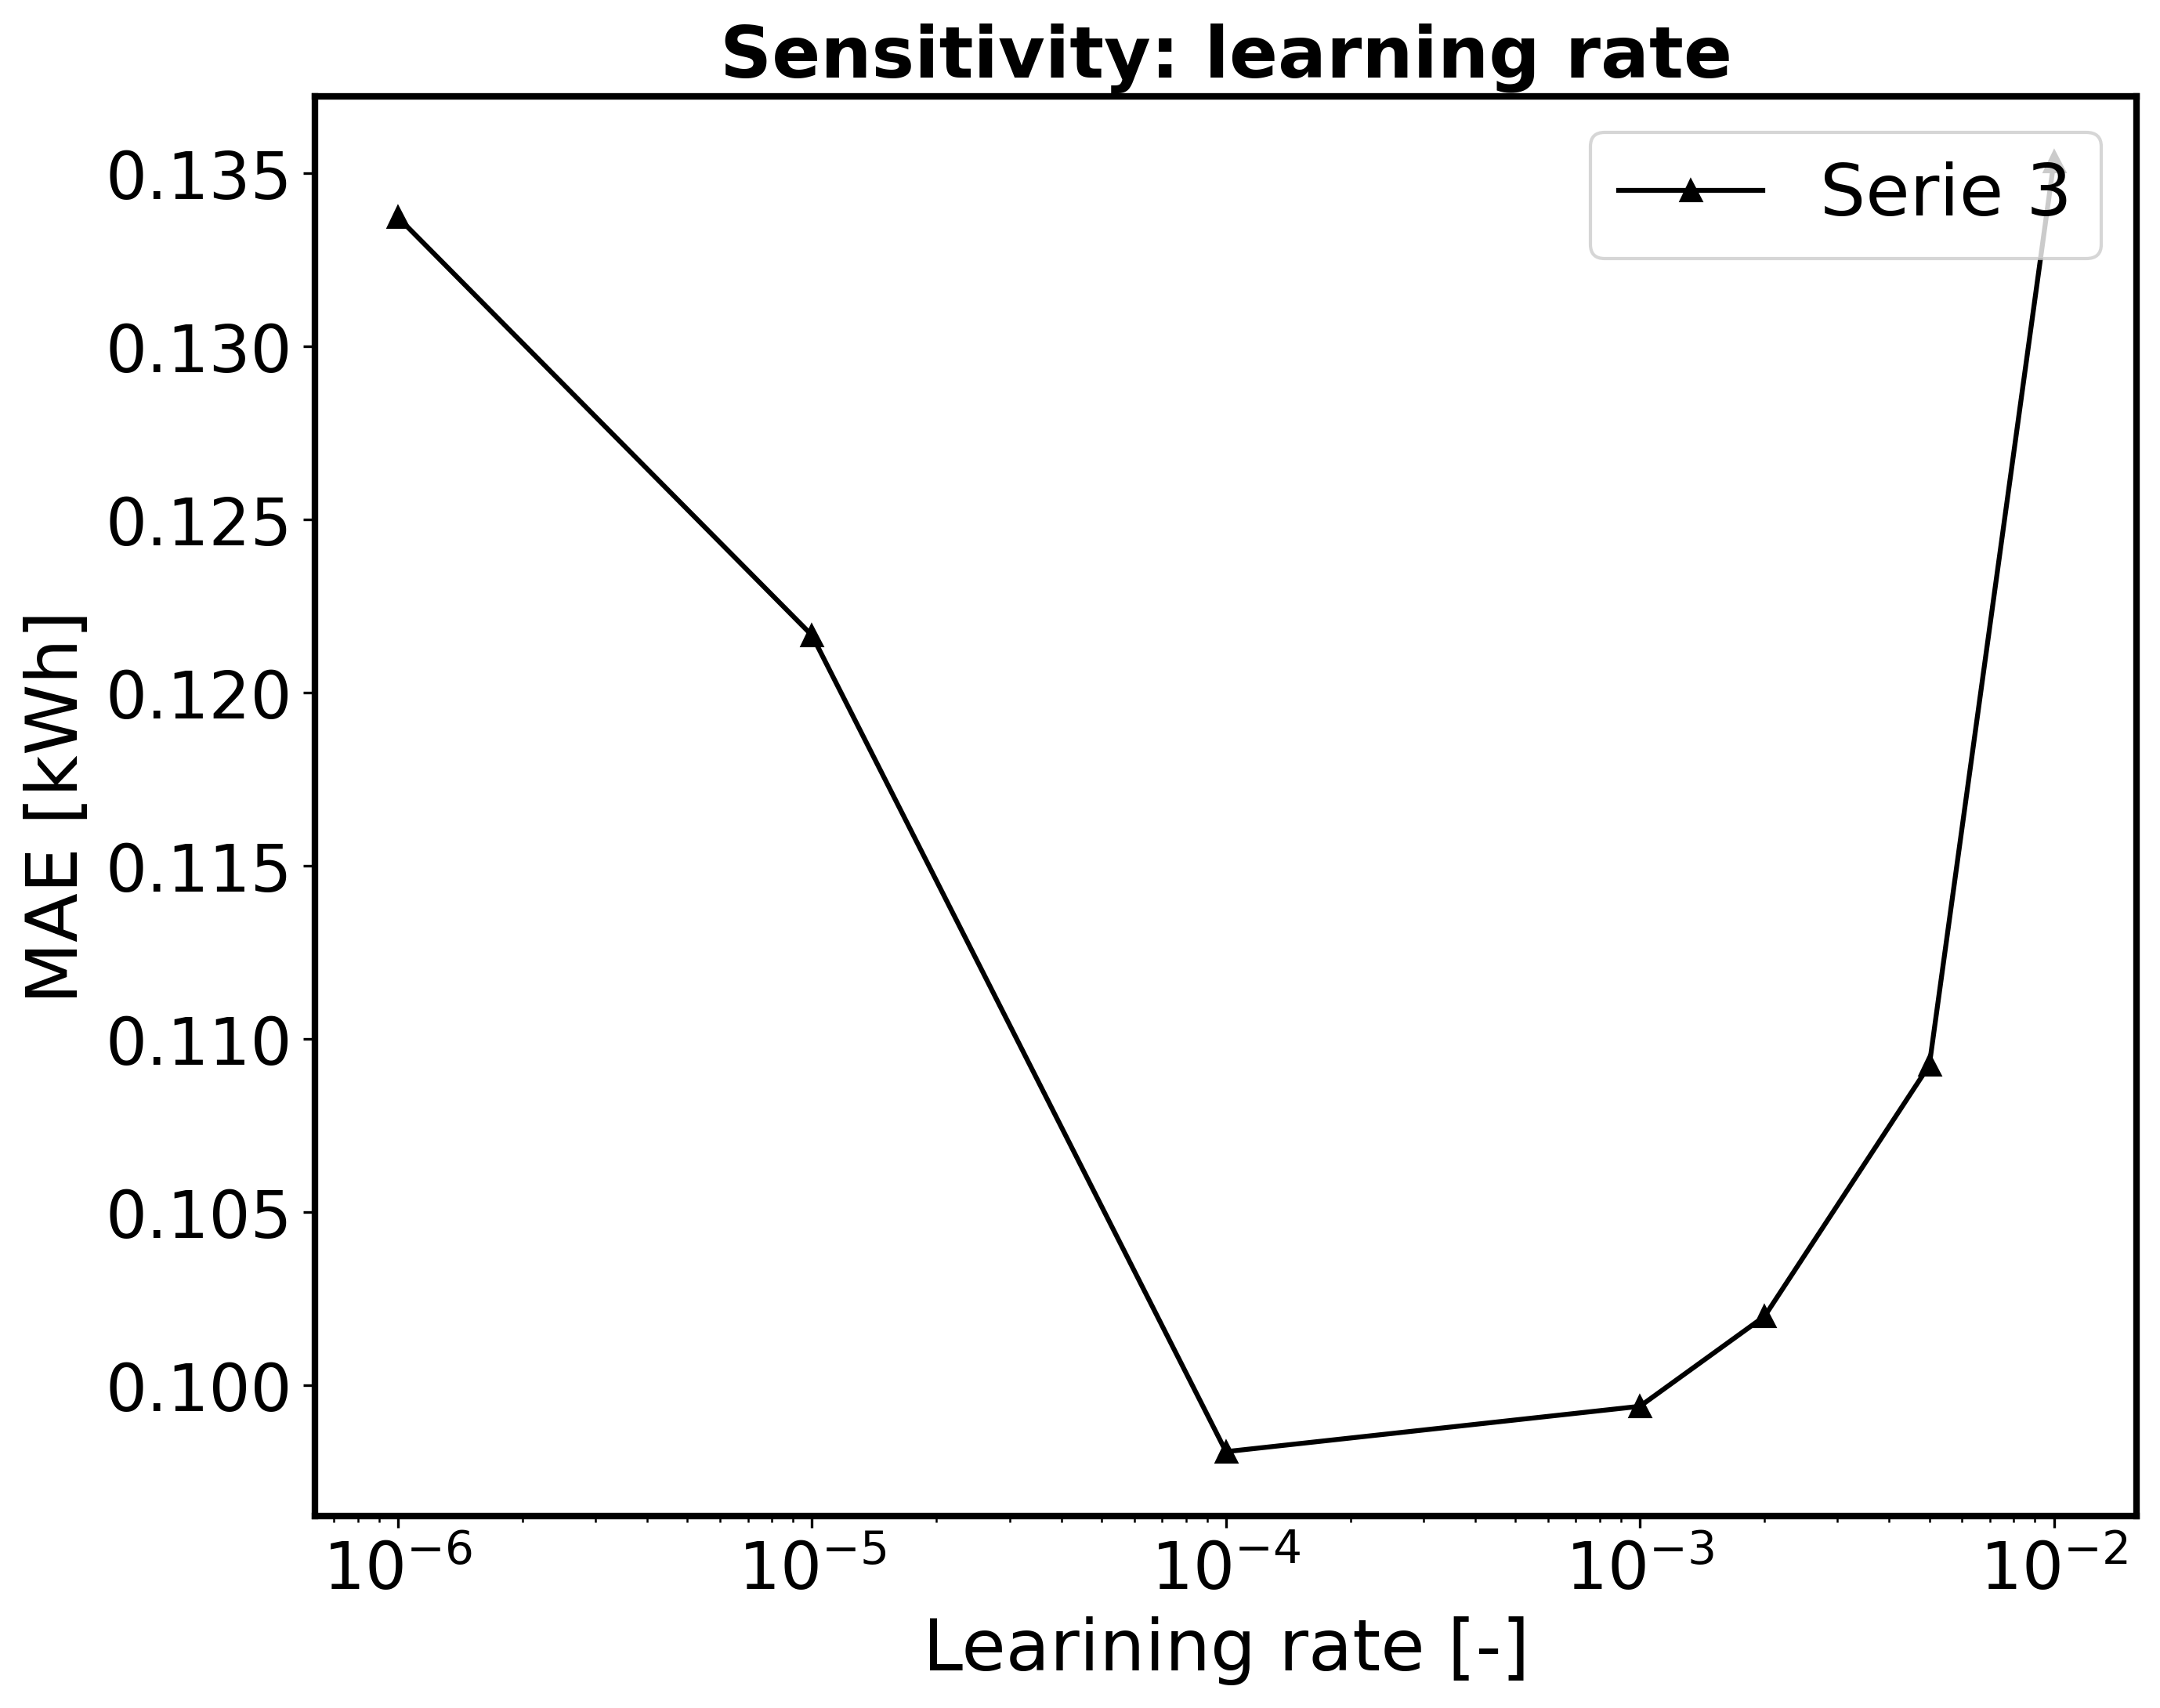
\includegraphics[width=1\linewidth]{learning_rate_serie3_model1.png}
		\caption{Model 1}
	\end{subfigure}
	\caption{The evaluation of the error on the validation set in function of the learning rate size.}
	\label{fig:learning_rate_model1}
\end{figure}


\textbf{Final model}\\
The final parameters for model one are displayed in Table \ref{tab:final_model1}.

\begin{table}[h]
	\centering
	\begin{tabular}{@{}l|ccc@{}} \toprule
		\multicolumn{4}{c}{Model 1: Stateless (no flatten layer)}\\\midrule\midrule
		\textbf{Parameters}	& \textbf{Serie $ 1 $} & \textbf{Serie $ 2 $} & \textbf{Serie $ 3 $}\\\midrule
		Units LSTM & $20 $&$ 50 $  & $50 $\\
		layers LSTM & $1 $&$ 3 $  & $3$\\
		Lag value & $96 $&$ 96$  & $48$\\
		Learning rate & $0.005 $&$ 0.0001$  & $0.0001$\\\hline
		Dropout inputs LSTM   & $ 0 $ & $ 0.2 $ & $ 0 $\\
		Dropout DENSE   & $ 0 $ & $ 0 $ & $ 0.4 $\\\bottomrule
	\end{tabular}
	\caption{Final values obtained after the parameter search for model 1.}
	\label{tab:final_model1}
\end{table}



\clearpage
\subsubsection{Model 2: Stateless with flatten layer}

\textbf{Phase 1}\\
The previous explained procedure is repeated for the other models. From Table \ref{tab:relative_performance_parameters_phase_one_model_two} it can again be seen that the choice of learning rate has the potential to give a big improvement and the use of an increased lag value of $ 96 $ didn't give a major improvement. 

\textbf{Phase 2}\\
From Figure \ref{fig:sensitivity_model2} it follows that:
\begin{itemize}
	\item Serie 1: The best setting after phase one and two is when a regularization parameter on the input weigh matrices is added of $ 10^{-5} $together with $ 3 $ LSTM layers and $ 50 $ hidden states. 
	\item Serie 2: The best setting after phase one and two is when a regularization parameter on the input weigh matrices is added of $ 10^{-3} $together with $ 3 $ LSTM layers and $ 50 $ hidden states.
	\item Serie 3: The best setting after phase one and two is when a dropout rate of $ 0.4 $ is added on the dense layer together with $ 3 $ LSTM layers and $ 50 $ hidden states.
\end{itemize}

\textbf{Phase 3}\\
Figure \ref{fig:learning_rate_model2} shows the sensitivity of the size of the learning rate in function of the MAE.

\textbf{Final model}\\
The final parameters for model two is displayed in Table \ref{tab:final_model2}.

\begin{table}[h]
	\centering
	\begin{tabular}{@{}l|ccc@{}} \toprule
		\multicolumn{4}{c}{Model 2: Stateless (no flatten layer)}\\\midrule\midrule
		\textbf{Parameters}	& \textbf{Serie $ 1 $} & \textbf{Serie $ 2 $} & \textbf{Serie $ 3 $}\\\midrule
		Units LSTM & $50 $&$ 50 $  & $50 $\\
		layers LSTM & $3 $&$ 3 $  & $3$\\
		Lag value & $96 $&$ 48$  & $96$\\
		Learning rate & $0.002 $&$ 10^{-5}$  & $0.0001$\\\hline
		Regularization on input weigh matrices LSTM   & $ 10^{-5} $ & $ 10^{-3} $ & $ 0 $\\
		Dropout DENSE   & $ 0 $ & $ 0 $ & $ 0.4 $\\\bottomrule
	\end{tabular}
	\caption{Final values obtained after the parameter search for model 2.}
	\label{tab:final_model2}
\end{table}

\newpage
\subsubsection{Model 3: Stateful model}
- Also one of the reasons that the stateful model performs better can be because there are a lot more weight updates because the weights are updated after each time step. Not True!! Batch size is still 48 --> but the lag value is one. 
- it seems reasonable to choose the batch size equal to 48 and not one. If one then focussed to much on the single values that have a lot of uncertainty on them. If you take 48, then you feed day per day and the whole day is looked at once, which is better to identify trends. 
- downside --> obtaining the predictions takes longer. For each prediction of a day the model is first seeded. 

The model is trained by making use of a batch size of one, which means that the weights of the LSTM block is updated by comparing each output immediately with its reference. \\

\textbf{Phase: 1}\\
During phase one the values chosen for the parameters as mentioned before, slightly different. The batch size and the lag value are both put to one. As can be seen in Figure \ref{tab:relative_performance_parameters_phase_one_model_three} the learning rate is still an important parameter to tune, but is also seen in Table \ref{tab:best_performing_para_phase1_model3} that one LSTM layer performed better than using three for the different series. 

\textbf{Phase: 2}\\
From Figure \ref{fig:sensitivity_model3} it follows that:
\begin{itemize}
	\item Serie 1: The best setting during phase one as shown in Table \ref{tab:best_performing_para_phase1_model3} outperformed all settings during phase two. 
	\item Serie 2: The best setting after phase one and two is when a regularization parameter on the hidden state weigh matrices is added of $ 10^{-3} $together with $ 3 $ LSTM layers and $ 50 $ hidden states.
	\item Serie 3: The best setting during phase one as shown in Table \ref{tab:best_performing_para_phase1_model3} outperformed all settings during phase two. 
\end{itemize}

It was found that the model when the three layers are used together with $ 50 $ hidden recurrent states, often produces a very big loss during training. If this is the case, the output of the training loss becomes not a number. Only for the regularizer on the recurrent hidden states of the LSTM and the regularizer on the inputs of the LSTM the results were better. The results of the two regularizers are shown in Figure \ref{fig:sensitivity_model3}.\\

As can be seen the parameter search of phase two for serie one and two performs worse than the parameter search of phase one. It is not necessarily the case that the addition of regularizers or dropout layers is the only cause of this bad behaviour. As could be seen in Tables \ref{tab:relative_performance_parameters_phase_one_model_three} and \ref{tab:best_performing_para_phase1_model3} one layer performed often better than three layers, which could also contribute to the worst results obtained during parameter search two. Only for serie 2 the best setting of phase one is outperformed. 

\textbf{Phase: 3}\\
Figure \ref{fig:learning_rate_model3} shows the sensitivity of the size of the learning rate in function of the MAE.

\textbf{Final model}\\
The final parameters for model two is displayed in Table \ref{tab:final_model3}.
\textbf{Remember to change the learning rates and the figures in appendix B...}
\begin{table}[h]
	\centering
	\begin{tabular}{@{}l|ccc@{}} \toprule
		\multicolumn{4}{c}{Model 3: Stateful}\\\midrule\midrule
		\textbf{Parameters}	& \textbf{Serie $ 1 $} & \textbf{Serie $ 2 $} & \textbf{Serie $ 3 $}\\\midrule
		Units LSTM & $50 $&$ 50 $  & $20 $\\
		layers LSTM & $1 $&$ 3 $  & $1$\\
		Lag value & $1 $&$ 1$  & $1$\\
		Learning rate & $ $&$ $  & $ $\\\hline
		Regularization on hidden states weigh matrices LSTM  & $ 0 $ & $ 10^{-3} $ & $ 0 $\\\bottomrule
	\end{tabular}
	\caption{Final values obtained after the parameter search for model 2.}
	\label{tab:final_model3}
\end{table}




\section{Conclusion}
This chapter discussed the data to perform the daily electricity consumption forecast on and which models are used. First, the baseline models were discussed. It was found that the mean forecast performed best for the error metrics: MAE, MSE, NRMSE and RMSE. ``MAPE forecast'' performed best when the MAPE error metric was considered. Both models predict the trend line and don't predict peaks in contrary to the closest day, 1 day and 7 days models. Next, the LSTM models that were developed were discussed. This included the practical considerations of the implementation of the models in Keras and a parameter search. The parameter search was done in three phases in order to reduce calculation load. It was found that the learning rate was the parameter that contributed the most to model performance.


%%% Local Variables: 
%%% mode: latex
%%% TeX-master: "thesis"
%%% End: 
